\chapter{Methodology}\label{ch:methodology}

In this study, we have considered the Agent-based simulation as our primary methodology for illustrating our supply chain model and accounting for disruptions. The supply chain model consists of 5 Suppliers, 7 Manufacturers, 10 Distributors, and 20 Retailers. Each facility acts as an individual agent which has been placed across the United States. The model represents the supply chain of one company having different facilities throughout the country. In the event of disruption, if any of the facilities gets shut down, then they have an alternative facility to turn to in order to get their demands satisfied. In the meantime, the facility that has been affected by the disruption is revived by taking the correct measures to increase the resiliency. Each facility has been assigned certain parameters of cost, time and demand fulfillment rate. There is a constant flow of materials downwards through the agents in the supply chain, while there is a constant flow of information upwards through the agents in the supply chain. It is important that this flow never breaks for the efficient performance of the system. In order to maintain this flow during disruption, alternate facilities are selected. The alternate facility gets selected based on the best parameter values amongst the available lists of facilities. There are a total of 5 scenarios depicting the source of disruption in the supply chain. The different strategies that need to be taken as per the source of the disruption are encompassed in the model for the purpose of restoration of the disrupted facility. The most efficient and appropriate strategy makes a massive impact on the resiliency of the system.


\newpage
\section{Agent-Based Modeling}

The main reason for developing the supply chain model as an agent-based simulation was due to the freedom to express the interaction between agents which is absolutely necessary to consider in our model. The complex nature of the supply chains makes it difficult to design models using the basic simulation models. Agent-based simulation helps in exhibiting the exact nature of a supply chain and all its players. The decision-making, information sharing, uncertainties, trade-offs, and coordination can be accurately represented by the agent-based simulation. It proves as the perfect platform to analyze different strategies and select the best one by implementing in the already existing model. The results are obtained at a fast rate and at an higher accuracy. 

\subsection{The Agents involved}

The model that we have developed for the purpose of our study contains four different agent types and are connected to each other for maintaining a sense of completion. Each agent type has a number of agents that are positioned across the United States of America. If the connections are lost, that means the supply chain has faced a disruption at some point in the network. The description of these agent types and the parameters associated with them are as follows.

\subsubsection{I. Supplier Agent}

These are the facilities that provide the raw materials to the manufacturing facility. In our model, there a total of 5 suppliers positioned across the country. The nomenclature for the suppliers has been done as S1, S2, S3, S4, and S5. The parameters associated with them are response time (time required to fulfill the demands of the manufacturer) and the raw material handling costs. The costs such as raw material handling cost and inventory holding costs are usually a percentage of the total costs. According to research, the percentage value for these costs lies between the range 40 to 60 percent of the total costs. The values of the parameters are as shown in the Table \ref{tab:Supplier}.

\begin{table}[H]
\caption{Parameters of the Supplier}
\label{tab:Supplier}
\begin{center}
\begin{tabular}[b]{|c|c|c|}
	\hline
	Supplier & Raw Material Handling Cost & Response Time \\ \hline
	S1 & 0.45 & High\\ \hline
	S2 & 0.52 & Medium \\ \hline
	S3 & 0.44 & High \\ \hline
	S4 & 0.58 & Low \\ \hline
	S5 & 0.56 & Medium \\ \hline
\end{tabular}
\end{center}
\end{table}

The values corresponding to the response time have ranking from 1 to 3. The rank 1 means that the response time is low, which is highly favorable for the selection criteria. Rank 2 and Rank 3 are the response time medium and high respectively. In the event of disruption, if a supplier is down, then alternate supplier is selected in such a way that the response time is either low or medium, and the raw material handling cost is the minimum.

\subsubsection{II. Manufacturer Agent}

Once the raw material has been acquired from the supplier, it comes to the manufacturer where it is converted into the final product. In our model, the 5 suppliers dispatch the raw materials to 7 manufacturers. These manufactures are positioned around the country and their nomenclature is done as M1, M2, M3,M4, M5, M6, and M7. The parameters associated with the manufacturer agents are inventory holding cost and response time. In the event of disruption, if any of the manufacturer that fulfills the demands of the distributors associated with it is down, then the alternate manufacturer is selected in such a way that the inventory holding cost is minimum, and the response time is either low or medium. The parameters for the manufacturer agent and their corresponding values are shown in the Table \ref{tab:Manufacturer}.


\begin{table}[H]
\caption{Parameters of the Manufacturer}
\label{tab:Manufacturer}
\begin{center}
\begin{tabular}[b]{|c|c|c|}
	\hline
	Manufacturer & Inventory Holding Cost & Response Time \\ \hline
	M1 & 0.51 & Low\\ \hline
	M2 & 0.41 & Medium \\ \hline
	M3 & 0.43 & Medium \\ \hline
	M4 & 0.57 & High \\ \hline
	M5 & 0.49 & Low \\ \hline
	M6 & 0.55 & High \\ \hline
	M7 & 0.48 & Low \\ \hline
\end{tabular}
\end{center}
\end{table}

\subsubsection{III. Distributor Agent}
The next agent is the distributor agent where the finished goods are collected from the manufacturer and are forwarded to the retailers. In our model we have 10 different distributors positioned across the country. The nomenclature for these 10 distributors is done as follows D1, D2, D3, D4, D5, D6, D7, D8, D9, and D10. The parameters associated with the distributors are inventory holding cost, order fulfillment rate, and response time. The selection of alternate distributor facility during disruption is done in such a way that the inventory holding cost should be minimum, order fulfillment rate should be high, and the response time should be low or medium. The parameters for the distributor agent and the values associated with them are as shown in the Table \ref{tab:Distributor}.


\begin{table}[H]
\caption{Parameters of the Distributor}
\label{tab:Distributor}
\begin{center}
\begin{tabular}[b]{|c|c|c|c|}
	\hline
	Distributor & Inventory Holding Cost & Order Fulfillment Rate & Response Time \\ \hline
	D1 & 0.46 & High & Medium\\ \hline
	D2 & 0.51 & High & High \\ \hline
	D3 & 0.44 & Low & Low \\ \hline
	D4 & 0.52 & High & High \\ \hline
	D5 & 0.48 & Low & Medium \\ \hline
	D6 & 0.49 & Low & Low \\ \hline
	D7 & 0.57 & High & Low \\ \hline
    D8 & 0.41 & High & Medium \\ \hline
    D9 & 0.48 & High & High \\ \hline
    D10 & 0.53 & Low & Low \\ \hline
\end{tabular}
\end{center}
\end{table}

\subsubsection{IV. Retailer Agent}
The fourth and final agent in our simulation model is the retailer agent. The retailers accrue the finished products from the distributors depending on the market trends and demands in their respective regions. In our model, there are a total of 20 retailers placed regionally across the country. Some regions have multiple retailers because of the high volume demand of the product from the customers. The nomenclature for the retailers are R1, R2, R3, R4, R5, R6, R7, R8, R9, R10, R11, R12, R13, R14, R15, R16, R17, R18, R19, and R20. A number of different retailer agents are connected to the same distributor agent. The parameter associated with the retailer agent is the response time (to the customers). The values corresponding to this parameter for the retailer agent is as shown in the Table \ref{tab:Retailer}.

\begin{table}[H]
\caption{Parameters of the Retailer}
\label{tab:Retailer}
\begin{center}
\begin{tabular}[b]{|c|c|}
	\hline
	Retailer & Response Time \\ \hline
	R1 & Low \\ \hline
	R2 & Medium \\ \hline
	R3 & Low \\ \hline
	R4 & High \\ \hline
	R5 & High \\ \hline
	R6 & Medium \\ \hline
	R7 & High \\ \hline
	R8 & Low \\ \hline
	R9 & Low \\ \hline
	R10 & Medium \\ \hline
	R11 & High \\ \hline
	R12 & Low \\ \hline
	R13 & Medium \\ \hline
	R14 & Medium \\ \hline
	R15 & High \\ \hline
	R16 & High \\ \hline
	R17 & High \\ \hline
	R18 & Low \\ \hline
	R19 & High \\ \hline
	R20 & Medium \\ \hline
\end{tabular}
\end{center}
\end{table}

\subsection{The Base Model Connections}
The four agent types are connected to each other to form 5 supply chains in the different regions throughout the country for a company. In the base model, the connections of the agents is as shown in the Fig.\ref{Base}. It can be observed from the Fig.\ref{Base} that the distributor D1 is shared by three retailers R3, R5 and R15. If there is a disruption in the area of Oregon and the distributor D1 is down due to it, then the retailers R3, R5, and R15 have to select a different distributor facility. They will choose the distributors from D2 to D10 based on who has the best parameter values. Similarly, the distributor agents and manufacturer agents connect to the best available manufacturer agent and supplier agent respectively based on the parameters. In the meantime, the restoration of the disrupted facility is taking place using appropriate mitigation strategies. This is the basic working logic of the whole simulation model.

\begin{figure}[H]
  \centering
  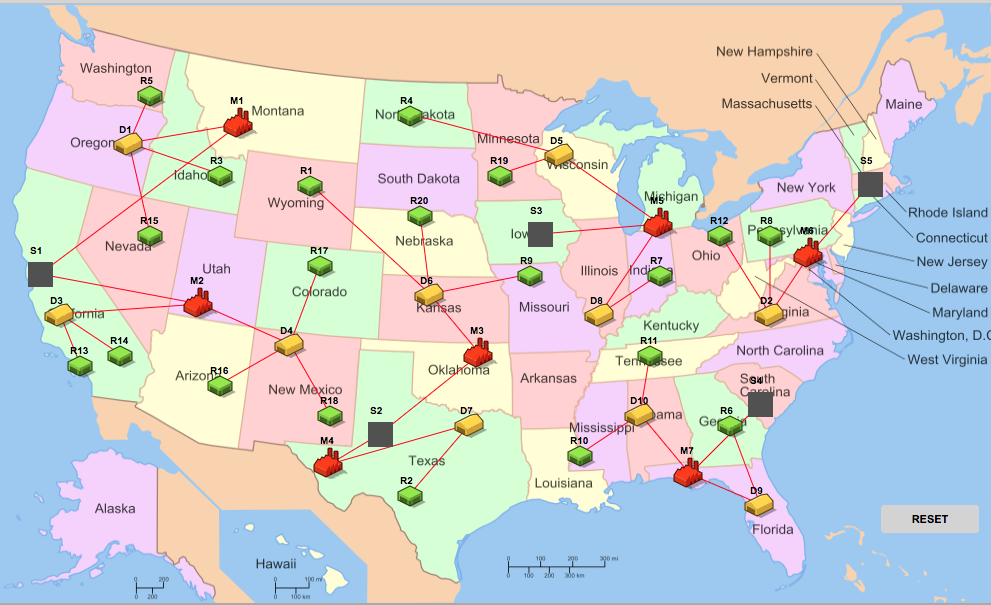
\includegraphics[width=6.5in]{figures/pdf/Basic-connections.png}\\
  \caption{Base Model Agent Connections.}\label{Base}
\end{figure}

\newpage
\section{Vulnerabilities and Capabilities}

There a lot of reasons for the disruptions to occur in the supply chain. Some may arise due to unfavorable natural conditions such as adverse weather, while some may be targeted attacks on firms. The knowledge of the source of disruption is very critical in order to devise proper mitigation strategies. If we know the reason of the disruption, then we can shift our focus on the repairing the most affected factors due to the disruption rather than doing the analysis of all the factors.

\begin{figure}[H]
  \centering
  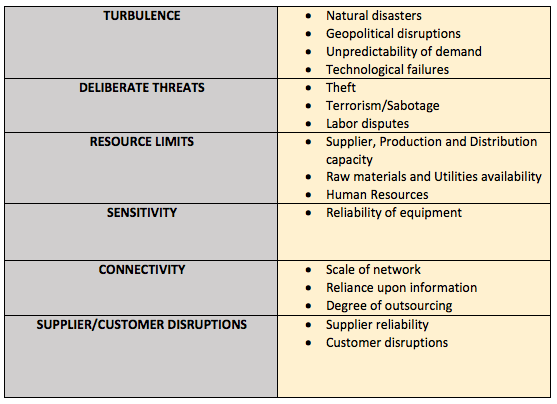
\includegraphics[width=6.0in]{figures/pdf/VNTS.png}\\
  \caption{Vulnerabilities and their various sources.}\label{Vulnerabilities}
\end{figure}

 \citep{Pettit2010} have jotted down these sources and factors as vulnerabilities and capabilities respectively. They have mentioned 7 vulnerabilities that lead to a disruption in the system. A firm should design its supply chain keeping in mind the relation between the vulnerabilities and capabilities. It should not have more capabilities as well as less capabilities. It should have just the perfect number of capabilities. If the company has enforced more capabilities, then there is a loss in capital. Also, if there are less capabilities, then the supply chain is left vulnerable to the disruptions.
 
We have implemented 6 out of the 7 vulnerabilities that act as a source of disruption. These vulnerabilities are as shown in the Fig.\ref{Vulnerabilities}. The major problem that occurs during resolving a disruption in a system is the time taken for thorough analysis of the root cause of the problem.

\begin{figure}[H]
  \centering
  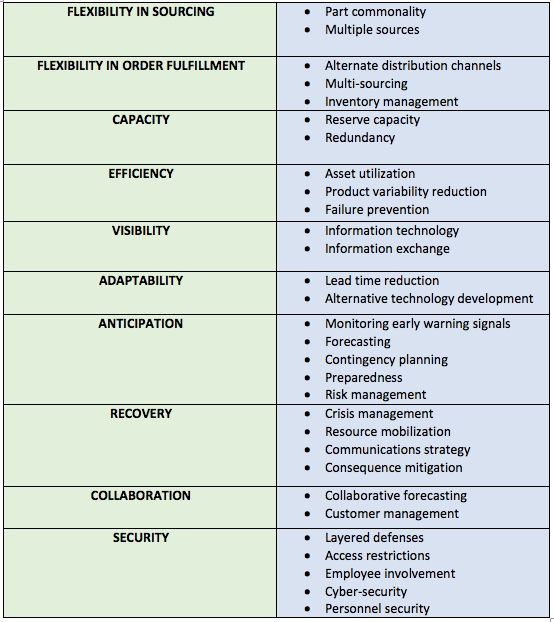
\includegraphics[width=6.0in]{figures/pdf/C1.png}\\
  \caption{Capabilities and their various types.}\label{Capabilities}
\end{figure}

 If the managers are well aware of the most common and recurring sources of disruption, they might be able to take preventive and reactive measures during disruptions of similar type in the future. By implementing these vulnerabilities in our supply chain design, we are not only providing ready measures of repair but also reducing the impact of disruption. Thus, making the system both resilient and robust in nature.  



\begin{figure}[H]
  \centering
  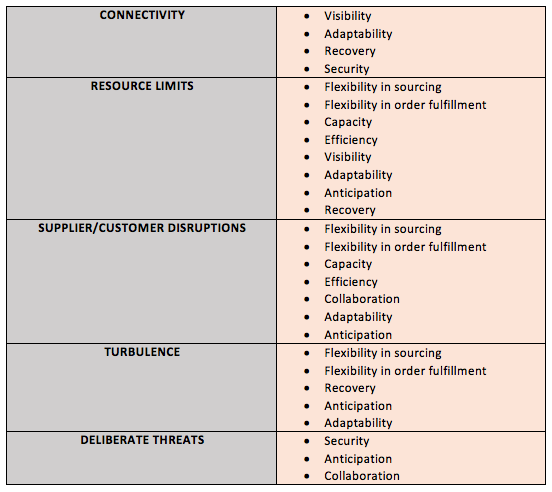
\includegraphics[width=6.0in]{figures/pdf/CV.png}\\
  \caption{Capabilities vs Vulnerabilities.}\label{CV}
\end{figure}


Once that the vulnerabilities are addressed, the next step is to glance at the capabilities (factors) that are most likely to be affected due to a certain kind of disruption rather looking at all the factors. This will help in reducing the time to find out where the exact problem lies. The list of capabilities that affect the performance of the supply chain system is as shown in Fig\ref{Capabilities}. These capabilities start to get damaged once the disruption occurs. The vulnerabilities that are closely associated with the capabilities are as shown in the Fig\ref{CV}. These prove to be beneficial in identifying the key factors that can help in improving the speed of recovery of the system back to its functioning state.


\section{Scenarios in the model}
In a typical supply chain, disruption can occur at any of the levels. Thus, we have developed the scenarios in such a way that the disruptions are occurring at the distributor level, manufacturer level, and the supplier. Also, for all the three events, we have considered the scenarios in which the disruptions are occurring due to the vulnerabilities that have been mentioned earlier. In total, there are 18 different scenarios and three scenarios for the disruption modeling without considering for resiliency design to quantify the need for our study.

\begin{figure}[H]
  \centering
  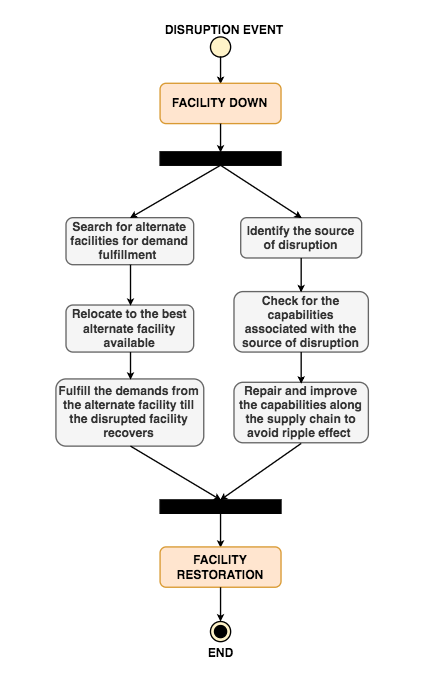
\includegraphics[width=2.0in]{figures/pdf/WL.png}\\
  \caption{Flowchart of Methodology.}\label{WL}
\end{figure}

 The working logic of the simulation model is as show in the Fig \ref{WL}. According to the logic, whenever the disruption occurs, the initial step is to identify the source of the disruption. The next step in the process is to check for the capabilities associated with the source of disruption that is most likely to get affected. During a disruption, it is not necessary that all the capabilities get damaged. Only a certain few capabilities get damaged which hinder with the performance of the system. The final step is to revive those damaged capabilities for getting the system functioning again.
 
The time between the occurrence of disruption and the identification of the key factors is called as the lost time ($T_{\text{L}}$). The time between the identification of the key factors and the total recovery of the disrupted facility is called as the recovery time $T_{\text{R}}$. The ratio of the recovery time to the lost time yields the resiliency percentage ($R_{\text{S}}$)  of the supply chain. 
 
 \begin{equation}
    Resiliency(R_S) = \frac{T_R}{T_L} \label{3.1}
\end{equation}

The higher the value of the resiliency, lesser is the length of recovery of the supply chain during disruption.

\subsection{Modeling without Resiliency and Robustness Consideration}
 In this model, the connections of the supply chain are as shown in the Fig\ref{Base}. There are three scenarios that can be observed for the behavior of supply chain under disruption. These scenarios are disruption at the distributor level, disruption at the manufacturer level, and disruption at the supplier level. Due to the absence of the key factor identification process in this model, a lot of time is wasted in finding out which factor of the supply chain is damaged which is hampering the entire system. Thus, the resiliency of the supply chain is going to have a lower value. 
 \subsubsection{Distributor Level Disruption}
 
 In this scenario, we have disrupted the distributor D3 which is located in the state of California. As the distributor D3 is down, it affects the other facilities associated with it. As a result, the demands from R13 and R14 retailers are not satisfied. A major backlog is recorder at these retailers due to the inability of those retailers to satisfy the customers in that area. The manufacturer M2 associated with the distributor D3 has to hold the inventory that was supposed to be delivered to the distributor. As the manufacturer is unaware of the duration of the recovery, it does not order any raw materials that were needed to manufacture the products that was supposed to be provided to the distributor. 
 
 \begin{figure}[H]
   \centering
    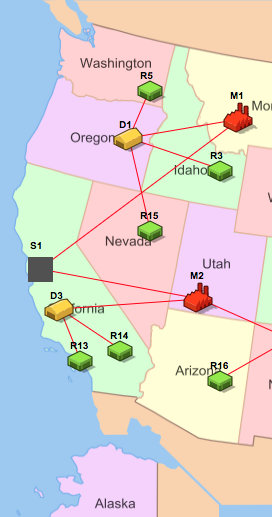
\includegraphics[width=1.5in]{figures/pdf/BeforeD.png} 
     \caption{Distributor Level Disruption (Before).}
     \label{fig:DLDb}
 \end{figure}
 
 \begin{figure}[H]
  \centering
  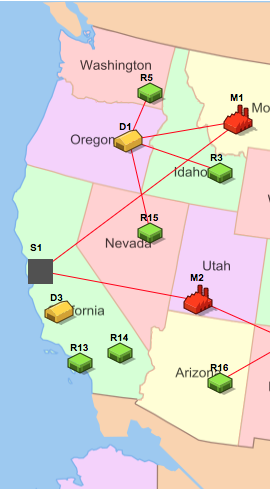
\includegraphics[width=1.5in]{figures/pdf/AfterD.png}
   \caption{Distributor Level Disruption (After).}
   \label{fig:DLDa}
\end{figure}

The connections before and after the disruption at the distributor D3 are shown in the Fig \ref{fig:DLDb} and Fig \ref{fig:DLDa}. It is evident from the figure that the disruption at the distributor causes D3 to disconnect from R13 and R14 retailers as well as M2 manufacturer.

\subsubsection{Manufacturer Level Disruptions}

In this scenario, we have disrupted the manufacturer M2 which is located in the state of Utah. As the manufacturer M2 is down, the effects of disruption spread throughout the supply chain through the facilities linked with it. As M2 is the manufacturer for two distributors D3 and D4, the two distributors are unable to collect the finished goods. As a result, the retailers R13, R14, R16, R17, and R18 are unable to fulfill the demands of the customers in their region. Thus, a backlog takes place both at the retailers and distributors. The supplier S1 linked to M2 has to hold the excess raw materials at their facility due to the uncertain duration of recovery of the disrupted facility. 

 \begin{figure}[H]
   \centering
    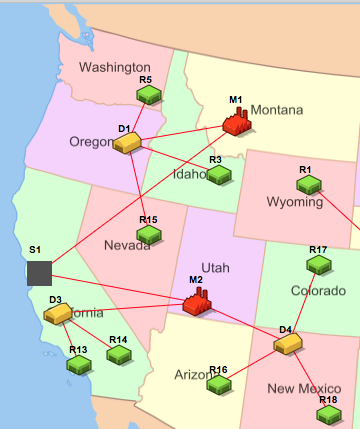
\includegraphics[width=2.0in]{figures/pdf/BeforeM.png} 
    \caption{Manufacturer Level Disruption (Before).}
    \label{fig:MLDb}
\end{figure}

\begin{figure}[H]
    \centering
   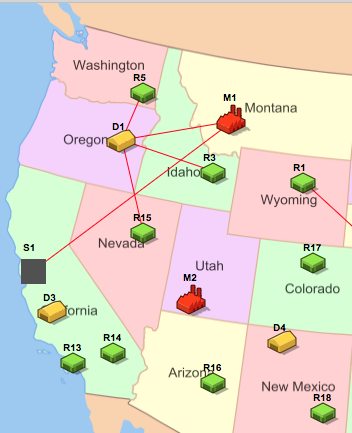
\includegraphics[width=2.0in]{figures/pdf/AfterM.png}
   \caption{Manufacturer Level Disruption (After).}
   \label{fig:MLDa}
\end{figure}

The connections before and after the disruption at M2 are shown in the Fig \ref{fig:MLDb} and Fig \ref{fig:MLDa}. The disruption causes the facilities R13, R14, R16, R17, R18, D3, and D4 to become inactive. The supplier S1 gets disconnected from the manufacturer M2.

\subsubsection{Supplier Level Disruption}

In this scenario, we disrupt the supplier facility S1 which is located in the state of California. Due to this, all the facilities that are linked to it get disrupted in one way or the other. The supplier S1 is the main and only provider of raw materials to the manufacturers M1 and M2. Thus the distributors and retailers associated with these two manufacturers have to wait for the S1 facility to recover from the disruption and provide the goods to the manufacturers so that they would be able to procure it from the manufacturers. 

\begin{figure}[H]
  \centering
  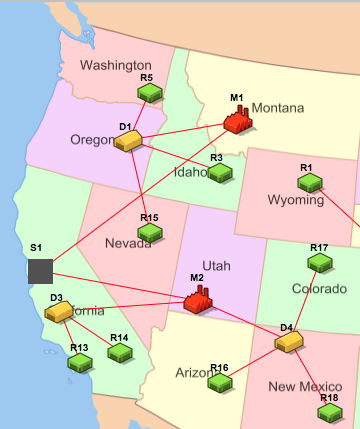
\includegraphics[width=2.5in]{figures/pdf/BeforeS.png}\\
  \caption{Supplier Level Disruption (Before).}\label{SLDB}
\end{figure}

\begin{figure}[H]
  \centering
  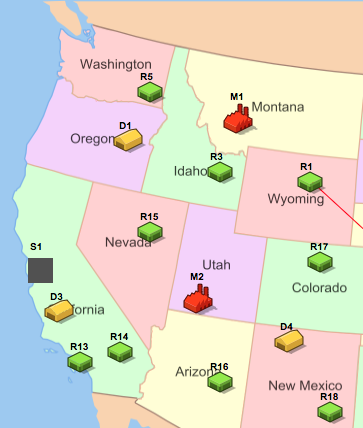
\includegraphics[width=2.5in]{figures/pdf/AfterS.png}\\
  \caption{Supplier Level Disruption (After).}\label{SLDA}
\end{figure}

In the Fig\ref{SLDB} the connections before the disruption at the supplier level are shown. The Fig\ref{SLDA} shows the disconnections caused due to the disruption at the supplier level. The facilities M1, M2, D1, D3, D4, R3, R5, R13, R14, R15, R16, R17 and R18 become inactive as they wait for the supplier S1 to recover from the disruption.

The lost time and recovery time occurred during different scenarios has a different value. Apart from the loss of time, there are other ramifications such as the backlog cost, inventory holding cost and the loss of customer loyalty. In this model the distributor level disruption causes a delay of a duration of 2 days. Out of this duration, the time for recovery ($T_{\text{R}}$) consisted of 12 hours while the lost time ($T_{\text{L}}$) was 36 hours. The resiliency of the model in this scenario is calculated as

\begin{equation}
    Resiliency(R_S) = \frac{12}{36} = 33.33 \% \label{3.2}
\end{equation}

The disruption at the manufacturer level causes a delay of 4 days in the supply chain. Out of these 4 days, the recovery time ($T_{\text{R}}$) is of 18 hours. The lost time ($T_{\text{L}}$) in this scenario is 78 hours. Thus, the resiliency of this scenario is even lesser than the previous scenario. It is calculated as

\begin{equation}
    Resiliency(R_S) = \frac{18}{78} = 23.07 \% \label{3.3}
\end{equation}

The disruption in the supplier level causes a delay of a week in the entire supply chain. The time for recovery ($T_{\text{R}}$) in this scenario is 24 hours, while the lost time ($T_{\text{L}}$) in this scenario is 144 hours. The resiliency of this scenario is calculated as

\begin{equation}
    Resiliency(R_S) = \frac{24}{144} = 16.66 \% \label{3.4}
\end{equation}

Among the three, the retailer level disruption scenario seems to have a better resilience value due to short difference of time between the lost time and the recovery time. It is to be noted that the duration of the disruption as well as the recovery time and lost time have been assumed. These values have been assumed so that the importance of implementing resilience and robustness in the supply chain can be quantified. There can be a huge variation in these values depending on the source of disruption. The values of resiliency obtained from the equations \ref{3.2}, \ref{3.3}, and \ref{3.4} are the values obtained during the disruption due to turbulence. Similarly, the values for resiliency of the system under different disruption sources can be obtained. The time lost ($T_{\text{L}}$) during these scenarios remains at all levels are the similar to that of the disruption due to turbulence. Thus the resiliency values for the other vulnerabilities that we have considered can be found out as well.

\subsubsection{Resiliency under disruption due to vulnerability due to Supplier/Customer Disruptions:}

\textit{At Distributor Level}
\begin{equation}
    Resiliency(R_S) = \frac{8}{36} = 22.22 \% \label{3.5}
\end{equation}
\newline
\textit{At Manufacturer Level}
\begin{equation}
    Resiliency(R_S) = \frac{14}{78} = 17.94 \% \label{3.6}
\end{equation}
\newline
\textit{At Supplier Level}
\begin{equation}
    Resiliency(R_S) = \frac{20}{144} = 13.88 \% \label{3.7}
\end{equation}

\subsubsection{Resiliency under disruption due to vulnerability due to Resource Limits:}

\textit{At Distributor Level}
\begin{equation}
    Resiliency(R_S) = \frac{6}{36} = 16.67 \% \label{3.8}
\end{equation}
\newline
\textit{At Manufacturer Level}
\begin{equation}
    Resiliency(R_S) = \frac{12}{78} = 15.38 \% \label{3.9}
\end{equation}
\newline
\textit{At Supplier Level}
\begin{equation}
    Resiliency(R_S) = \frac{18}{144} = 12.5 \% \label{3.10}
\end{equation}

\subsubsection{Resiliency under disruption due to vulnerability due to Connectivity:}

\textit{At Distributor Level}
\begin{equation}
    Resiliency(R_S) = \frac{11}{36} = 30.56 \% \label{3.11}
\end{equation}
\newline
\textit{At Manufacturer Level}
\begin{equation}
    Resiliency(R_S) = \frac{17}{78} = 21.79 \% \label{3.12}
\end{equation}
\newline
\textit{At Supplier Level}
\begin{equation}
    Resiliency(R_S) = \frac{23}{144} = 15.97 \% \label{3.13}
\end{equation}

\subsubsection{Resiliency under disruption due to vulnerability due to Deliberate Threats:}

\textit{At Distributor Level}
\begin{equation}
    Resiliency(R_S) = \frac{10}{36} = 27.78 \% \label{3.14}
\end{equation}
\newline
\textit{At Manufacturer Level}
\begin{equation}
    Resiliency(R_S) = \frac{16}{78} = 20.51 \% \label{3.15}
\end{equation}
\newline
\textit{At Supplier Level}
\begin{equation}
    Resiliency(R_S) = \frac{22}{144} = 15.27 \% \label{3.16}
\end{equation}


Thus, there arises a need for designing a supply chain with resilience and robustness incorporated in it as there is a huge scope in reducing the time lost in recognizing the key indicators of the system. 


\subsection{Modeling with Resiliency and Robustness Consideration}

In this model, we have implemented the key indicator identification and contingency planning components into our supply chain. Whenever a disruption takes place, the source of the disruption is identified and a team of management personnel look into the capabilities that are most probable of being affected. In the meantime, an alternate facility having the lowest costs, high fulfillment rate, and low response time is selected from the other available facilities. There is transportation cost that is incurred due to alternate facility location. But, this cost is just a small price to pay in order to avoid huge losses if we wait for the damaged facility to be repaired. The lost time is reduced by a drastic amount and thus the total delay caused by the disruption is reduced while keeping the supply chain working simultaneously. Thus, a resilient and robust supply chain is achieved.

\subsubsection{SCENARIO I: Disruptions due to Turbulence}

In this scenario we have identified the source of disruption as turbulence. Theses disruptions are mainly caused by natural disasters, geopolitical disruptions, unpredictability of demand, and technological failures. As the source of disruption is identified, the capabilities associated can be inspected for the damages and the process of repairing the damages can be initiated for getting a rapid recovery. The key indicators identified during this type of disruption are flexibility in sourcing, flexibility in order fulfillment, recovery, anticipation, and adaptability. The disrupted facilities are the same as the previous model for the sole reason of comparison of the values obtained in the resiliency. Thus, signifying the need for resiliency and robustness in the supply chain design.

\subsubsection{Distributor Level Disruption}
In this part of scenario I, we are targeting the distributor D3 in the state of California. The moment the distributor D3 is down due to the disruption, with the help of contingency planning, an alternate distributor is selected for fulfilling the demands of the retailers R13 and R14. Thus, the supply chain has a continuous functionality. As we the source of the disruption is comprehended, the problems are identified much quicker. The recovery time also becomes lesser as we have the knowledge of what strategies need to be considered for improving the capabilities. Thus, the total down time of the facility is reduced by a substantial amount.

\begin{figure}[H]
  \centering
  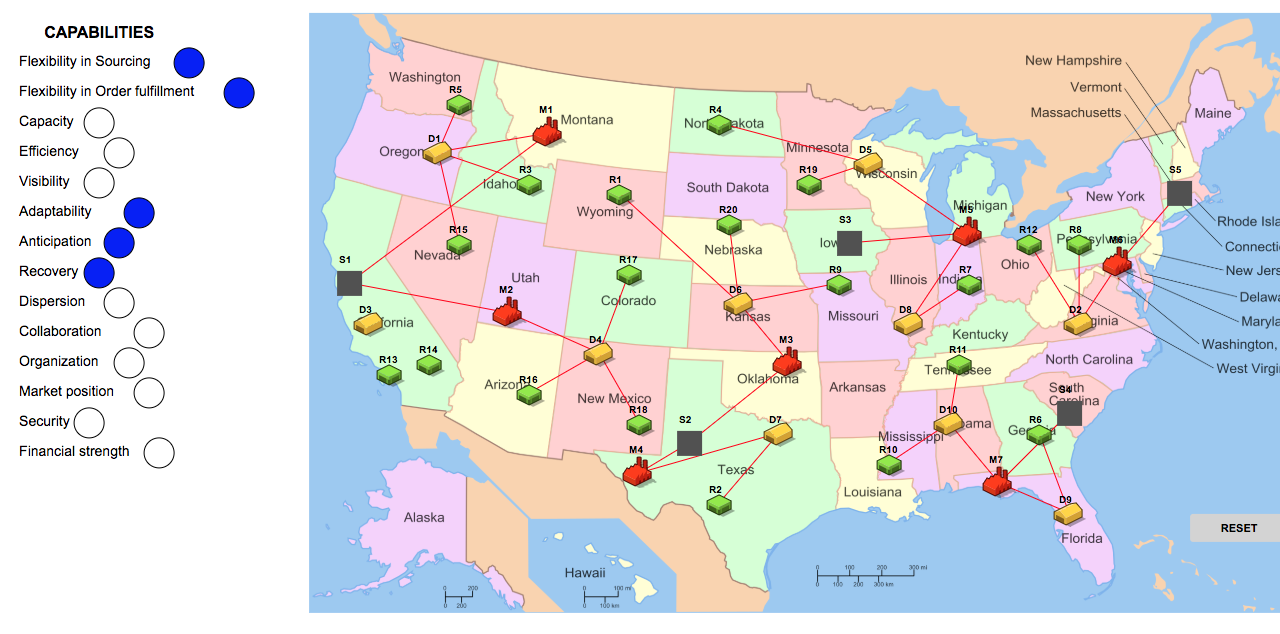
\includegraphics[width=6.5in]{figures/pdf/Scenario1DLD.png}\\
  \caption{Scenario I (Distributor Level Disruption).}
  {The distributor D3 is getting disrupted due to which the retailers associated with it are left unsatisfied. The manufacturer facility M2 is holding the inventory required by the disrupted facility D3. The capabilities associated with this type of disruption are being identified.}
  \label{SID}
\end{figure}

The Fig \ref{SID} shows the disrupted distributor D3 and the loss of its connection with the manufacturer M2, retailer R13, and retailer R14. The key indicators being identified can also be observed in this figure. The alternate distributor facility are selected for the retailers R13 and R14. There are three options that are selected by the simulation after putting the constraints as low or medium response time, high fulfillment rate, and minimum inventory holding cost. These distributor facilities are D1, D7 and D8 and the connections of the retailers R13 and R14 are as show in the Fig \ref{ALTD}. Out of these options, D1 is the best choice due to the proximity to the retailers. The transportation cost incurred would be lesser than the other two facilities.                                                            

\begin{figure}[H]
  \centering
  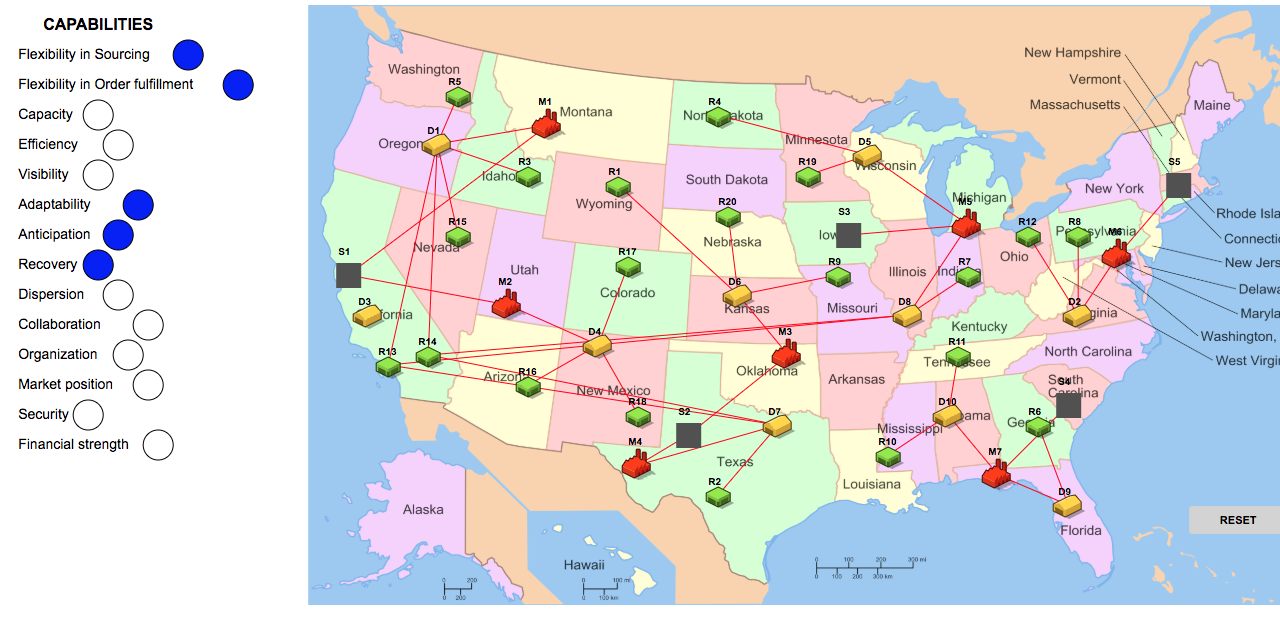
\includegraphics[width=6.5in]{figures/pdf/ALTD.png}\\
  \caption{Alternate Distributor Facility Selection Options for R13 and R14 retailers.}
  {The alternate distributor facilities D1, D7 and D8 are being selected as the possible options for the retailers R13 and R14 to maintain the continuous functioning state of the supply chain.}
  \label{ALTD}
\end{figure}                                                                                                            The lost time ($T_{\text{L}}$)  that is recorder in this scenario has been reduced to 18 hours due to the implementation of identification technique and contingency planning. The time for recovery ($T_{\text{R}}$) remains the same as 12 hours. Thus, the resiliency of the model appears to be having a higher value.

\begin{equation}
    Resiliency(R_S) = \frac{12}{18} = 66.67 \% \label{3.17}
\end{equation}

In this scenario, due to the contingency planning, the down time of the distributor does not cause any hampering effects on the other facilities associated with it. This is due to the retailers associated with the disrupted facility are allocated a different distributor that has the capability to fulfill their demands. However, the manufacturer facility M2 has to wait for the distributor D3 to be repaired. But, the waiting time is reduced in this scenario. Thus, the inventory holding cost will not be as much as in the scenario without resiliency consideration. Once the disrupted facility is repaired, the network gets back to its original state as shown in Fig \ref{Base}. 


\subsubsection{Manufacturer Level Disruption}

In this part of scenario I, an event is created where the manufacturer facility M2 is disrupted. The distributors associated with this facility disconnect from M2. The retailers connected to those distributors become inactive due to the disruption. The contingency planning comes into action here and the distributors D3 and D4 are relocated to other available manufacturers. Their retailers become active once they get relocated to different facilities. The effect of the manufacturer level disruption on the supply chain is as shown in the Fig \ref{S1MLD}. 

\begin{figure}[H]
  \centering
  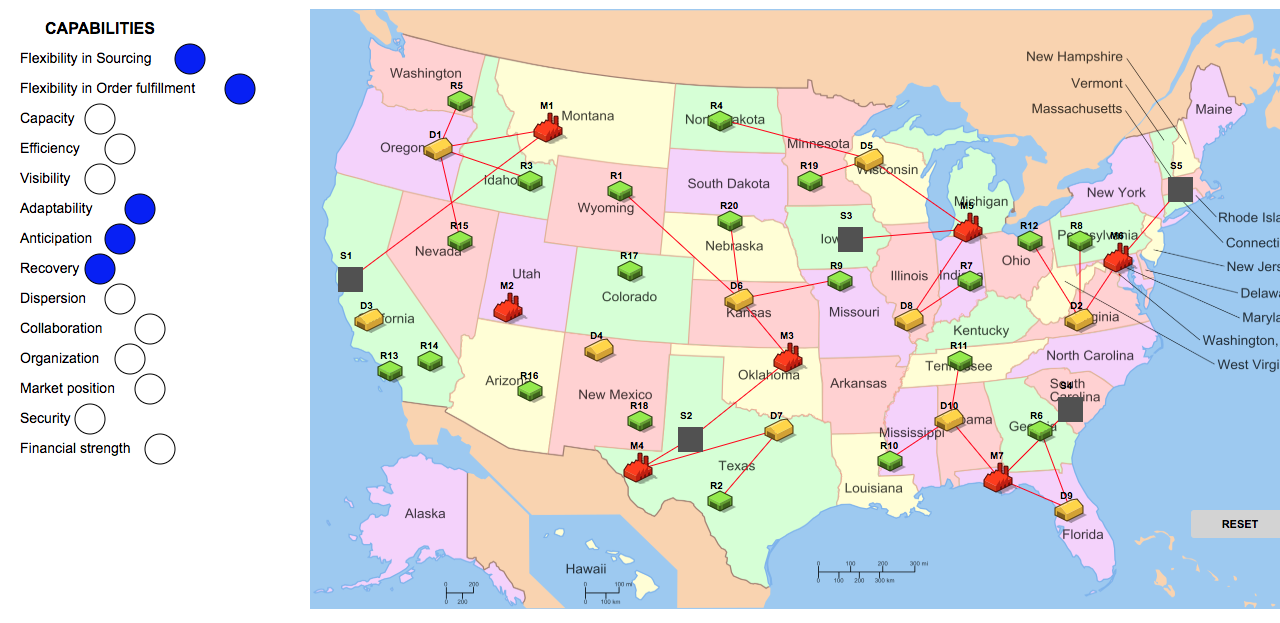
\includegraphics[width=6.5in]{figures/pdf/S1MLD.png}\\
  \caption{Scenario I (Manufacturer Level Disruption).}
  {The manufacturer M2 is getting disrupted due to which the  distributors and retailers associated with it are left unsatisfied. The supplier facility S1 is holding the inventory required by the disrupted facility M2. The capabilities associated with this type of disruption are being identified.}
  \label{S1MLD}
\end{figure}    

Through the contingency planning, the simulation software selects three options available for the relocation of the distributors D3 and D4. These selections are based on the constraints of low inventory holding cost and  low/medium response time. These manufacturing facilities are M3, M5, and M7 and are as shown in the Fig \ref{ALTM}. Out of these alternatives, the facility M3 has an advantage over the others in terms if inventory holding cost and transportation cost. 

\begin{figure}[H]
  \centering
  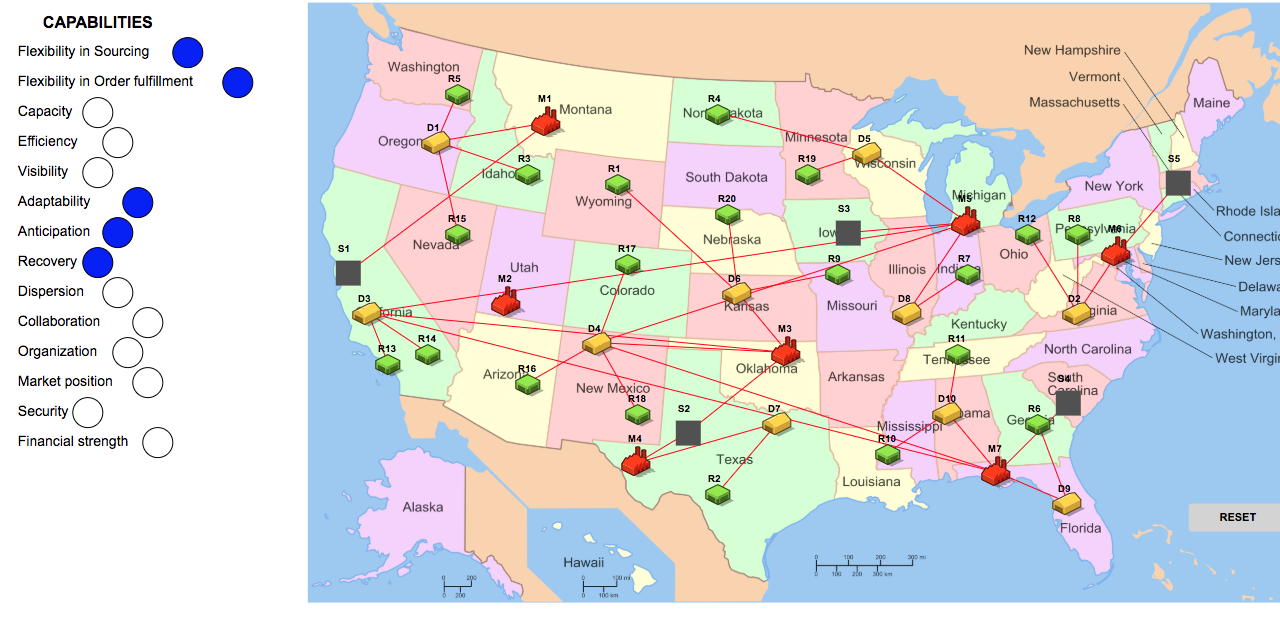
\includegraphics[width=6.5in]{figures/pdf/ALTM.png}\\
  \caption{Alternate Manufacturer Facility Selection Options for D3 and D4 distributors.}
  {The alternate manufacturer facilities M3, M5 and M7 are being selected as the possible options for the distributors D3 and D4 to maintain the continuous functioning state of the supply chain.}
  \label{ALTM}
\end{figure}    

During the alternate sourcing of the manufacturers for D3 and D4, the facility M2 is in the repairing process with the help of key indicator identifications. The lost time ($T_{\text{L}}$) is reduced as well due to these identification strategies and is now 54 hours instead of 78 hours. The recovery time ($T_{\text{R}}$) remains the same as it is dependent on the source of disruption. The resiliency of the supply chain in this scenario has increased due to the reduction in the lost time ($T_{\text{L}}$) in the system. 

\begin{equation}
    Resiliency(R_S) = \frac{18}{54} = 33.33 \% \label{3.18}
\end{equation}

The contingency planning does not allow any discontinuities to take place in the supply chain. The distributors fulfill their demands from the manufacturer M3 till the facility M2 recovers from the disruption. When M2 is fully recovered, the distributors go back to their original manufacturers. Thus, the supply chain gets back to its original functioning state. 

\newpage
\subsubsection{Supplier Level Disruption}

The supplier level disruption contains an event that destroys the facility S1 and all the facilities connected to them get disrupted as well. This scenario has the most damaging effect on the supply chain as it can get the entire system come to a standstill. The manufacturers M1 and M2 are disconnected and therefore the distributors D1, D3 and D4 are disconnected as well. As a result, the retailers associated with these distributors are unable to satisfy the customer demands in their region. The effect of the supplier level disruption and the key factors identification in the supply chain is as shown in the Fig \ref{S1SD}.

\begin{figure}[H]
  \centering
  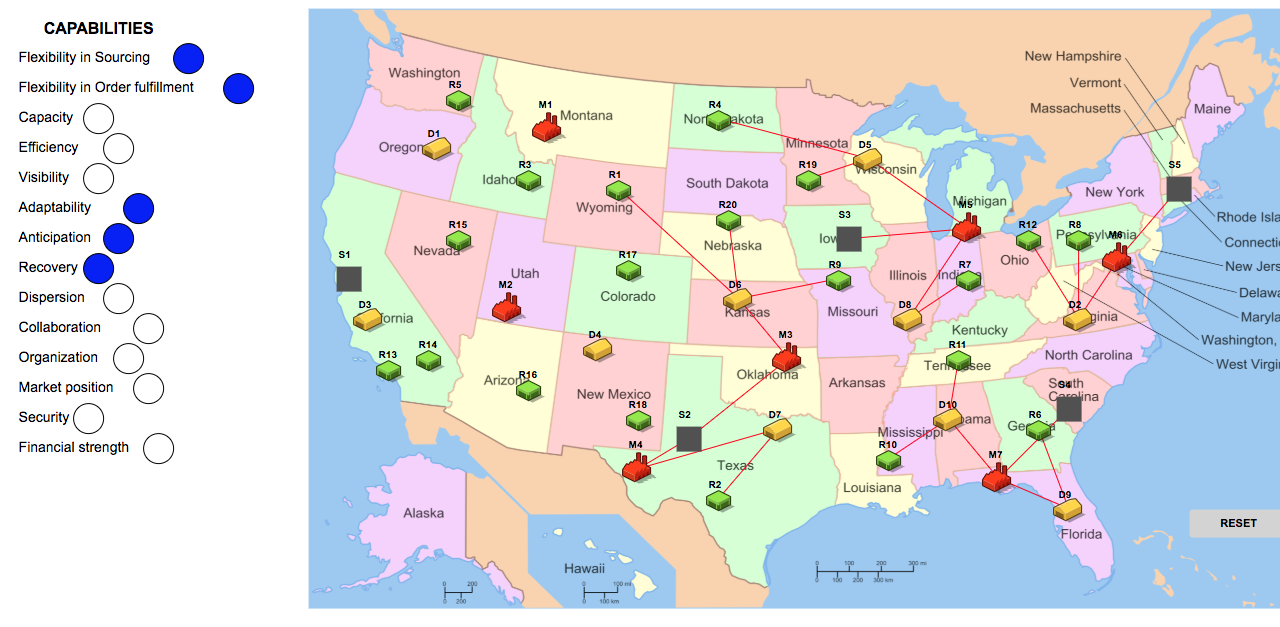
\includegraphics[width=6.5in]{figures/pdf/S1SLD.png}\\
  \caption{Scenario I (Supplier Level Disruption).}
   {The Supplier S1 is getting disrupted due to which the manufactures, distributors, and retailers are left unsatisfied. The entire supply chain is waiting for the facility S1 to be recovered for gaining back the functionality. The capabilities associated with this type of disruption are being identified.}
  \label{S1SD}
\end{figure}    

The entire supply chain gets disrupted when the S1 facility is disrupted. The key indicators are identified and the recovery process is initialized. With the help of contingency planning, the distributors are relocated to other available suppliers. The simulation tool aids us in finding the best supplier in terms of cost and response time. The constraints considered in the selection criteria are low raw material handling cost and low response time. There is only one supplier which meets the provided constraints. This supplier is the facility S4 and the alternate selection done by the simulation software is as shown in the Fig \ref{ALTS}.

\begin{figure}[H]
  \centering
  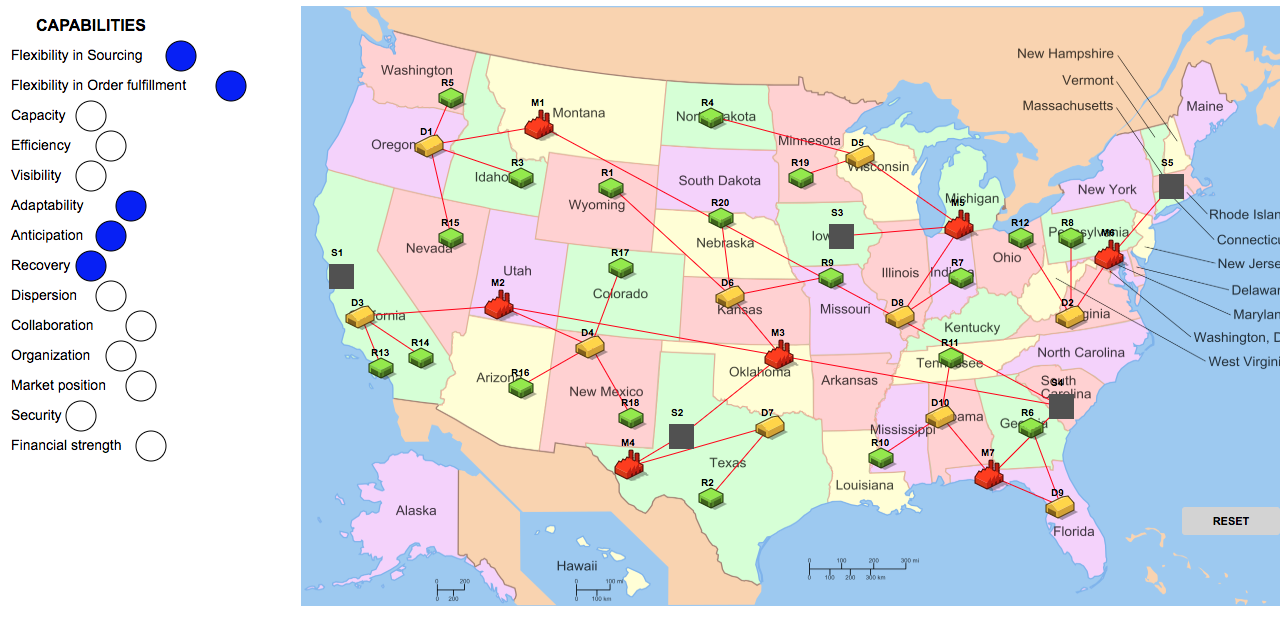
\includegraphics[width=6.5in]{figures/pdf/ALTS.png}\\
  \caption{Alternate Supplier Facility Selection Options for M1 and M2 manufacturers.}
  {The alternate supplier facility S4 is being selected for the manufacturers M1 and M2 to maintain the continuous functioning state of the supply chain.}
  \label{ALTS}
\end{figure}    

The manufacturing facilities M1 and M2 acquire the raw materials from the new supplier S4 till the disrupted facility S1 is recovered completely. Once the facility S1 is restored, the supply chain gets back to its original state.
The lost time ($T_{\text{L}}$) observed here is reduced by a huge amount to 96 hours from the original 144 hours. The recovery time still remains the same as the source of disruption is considered the same. The recovery time ($T_{\text{R}}$) value is 24 hours. The resiliency of the system is increased due to the reduction in the lost time. 

\begin{equation}
    Resiliency(R_S) = \frac{24}{96} = 25.00 \% \label{3.19}
\end{equation}

The inventory holding costs, loss of customer loyalty, and the backlog costs are eliminated due to incorporating the contingency planning and key indicators identification. Thus, the supply chain becomes resilient to disruptive events and becomes robust in the face of an uncertainty.

\newpage
\subsubsection{SCENARIO II: Supplier/Customer Disruptions}

This scenario encompasses the supplier/customer disruptions which occur very frequently. The main sources of this type of disruption are supply reliability and customer disruptions. Since we know the source of disruption, the key indicators (capabilities) are investigated and the recovery process can get underway. These key indicators are flexibility in sourcing, flexibility in order fulfillment, capacity, efficiency, collaboration, adaptability, and anticipation. Again, the disrupted facilities are kept same for the purpose of observing the performance of supply chain with and without contingency planning and key indicators identification. 

\subsubsection{Distributor Level Disruption}

\begin{figure}[H]
  \centering
  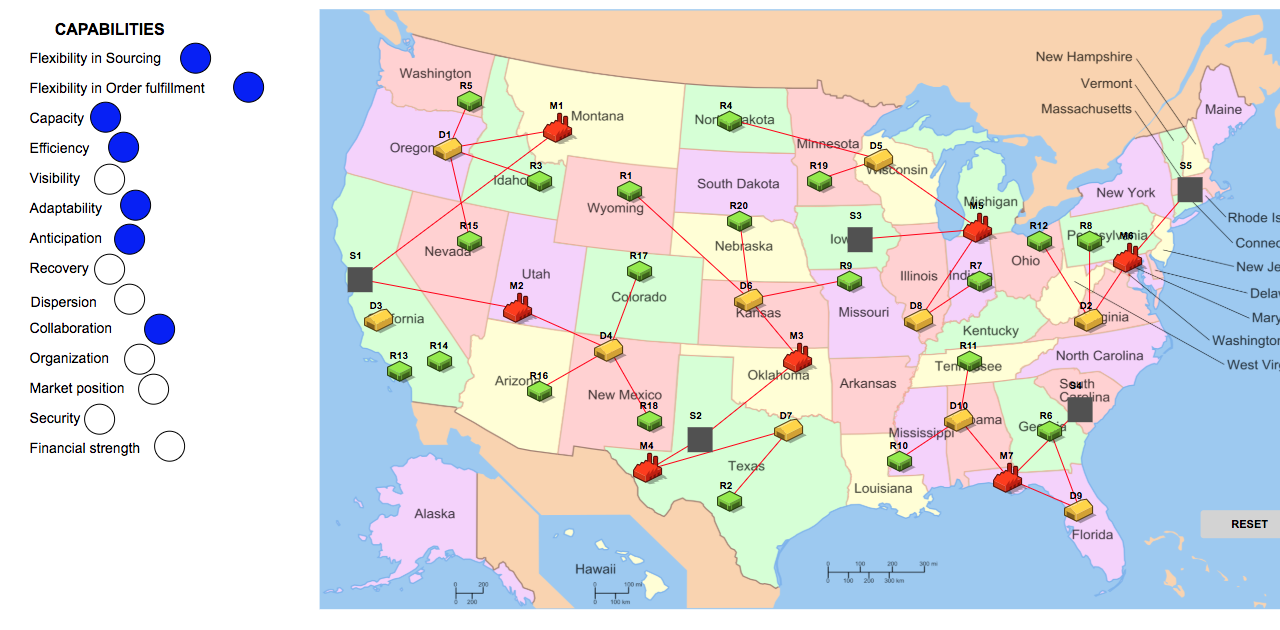
\includegraphics[width=6.5in]{figures/pdf/S2DLD.png}\\
  \caption{Scenario II (Distributor Level Disruption)}
  {The distributor D3 is getting disrupted due to which the retailers associated with it are left unsatisfied. The manufacturer facility M2 is holding the inventory required by the disrupted facility D3. The capabilities associated with this type of disruption are being identified.}
  \label{S2DL}
\end{figure}   

The Fig \ref{S2DL} shows the disruption occurring at the distributor level and the D3 facility is down. The retailers R13 and R14 along with the manufacturer M2 gets disconnected from D3. The cause of this uncertainty is the supplier/customer disruption and the key indicators associated with it are immediately addressed. The recovery process starts as soon as these capabilities are addressed. The alternate facility selection is the same as that of fig \ref{ALTD}. Thus, the lost time ($T_{\text{L}}$) is reduced due to the identification of the key capabilities. The time to recovery ($T_{\text{R}}$) remains the same as that of equation \ref{3.5}. The resiliency of this scenario is therefore increased.

\begin{equation}
    Resiliency(R_S) = \frac{8}{18} = 44.44 \% \label{3.20}
\end{equation}

By the introduction of contingency planning and key indicators identification into the supply chain design, the resiliency of supply chain was increased from 22.22 \% to 44.44 \% .

\subsubsection{Manufacturer Level Disruption}

\begin{figure}[H]
  \centering
  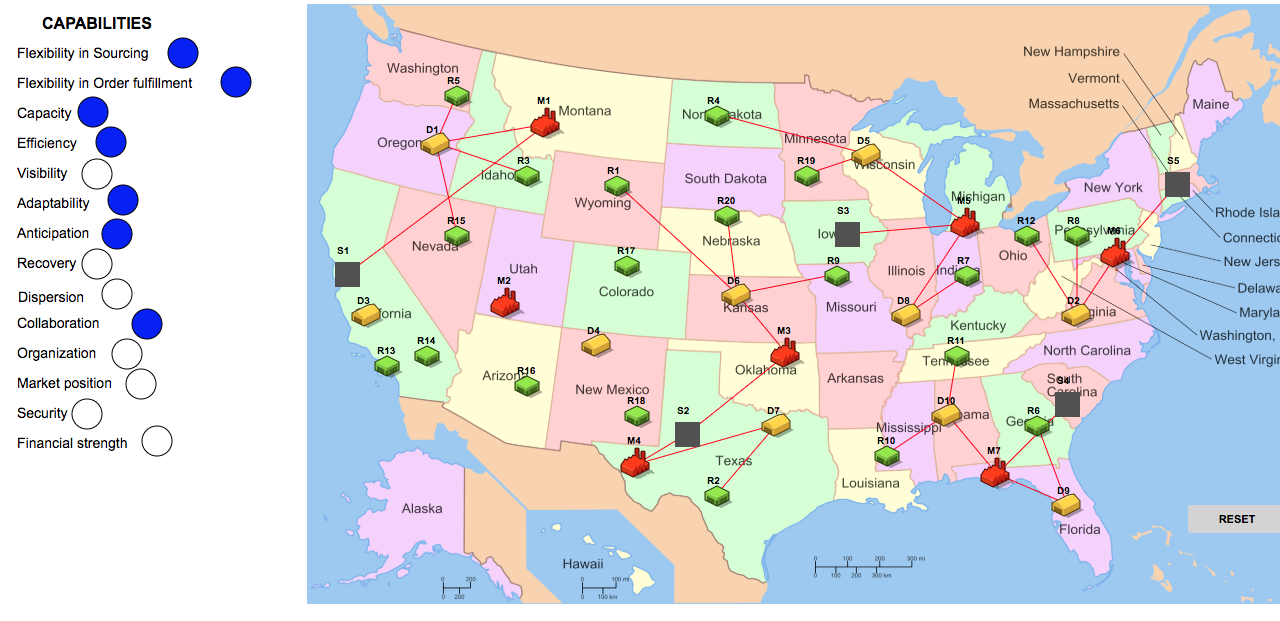
\includegraphics[width=6.5in]{figures/pdf/S2MLD.png}\\
  \caption{Scenario II (Manufacturer Level Disruption)}
  {The manufacturer M2 is getting disrupted due to which the  distributors and retailers associated with it are left unsatisfied. The supplier facility S1 is holding the inventory required by the disrupted facility M2. The capabilities associated with this type of disruption are being identified.}
  \label{S2ML}
\end{figure}   

The Fig \ref{S2ML} shows the disruption occurring at the manufacturer M2 causing the facilities D3, R13, R14, R16, R17, R18, D4 and S1 to disconnect from it. The raw materials are held up at the S1 facility till the facility M2 gets recovered, while the facilities D3 and D4 are inactive due to no supply of the materials to them. The identification of the key indicators help in resolving the issues caused due to the disruption at a faster rate. Thus, the lost time ($T_{\text{L}}$) is reduced while the recovery time ($T_{\text{R}}$) remains the same as that of equation\ref{3.6}. The resiliency of this system is comparatively better than that of the system without resiliency and robustness consideration. The contingency planning allocates an alternate manufacturing facility for D3 and D4 in the similar way as shown in Fig \ref{ALTM} till the M2 facility recovers. 

\begin{equation}
    Resiliency(R_S) = \frac{14}{54} = 25.92 \% \label{3.21}
\end{equation}

With the help of the resiliency and robustness consideration, the resiliency of the system in this scenario is increased from 17.94 \% to 25.92 \% .

\subsubsection{Supplier Level Disruption}

\begin{figure}[H]
  \centering
  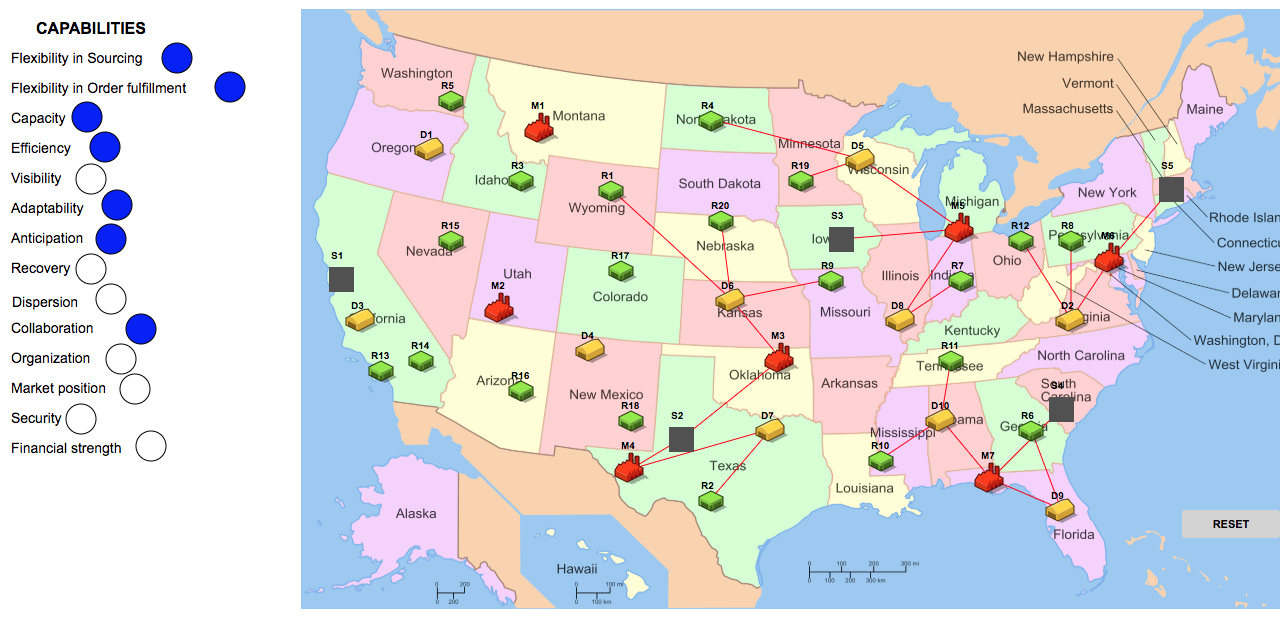
\includegraphics[width=6.5in]{figures/pdf/S2SLD.png}\\
  \caption{Scenario II (Supplier Level Disruption)}
   {The Supplier S1 is getting disrupted due to which the manufactures, distributors, and retailers are left unsatisfied. The entire supply chain is waiting for the facility S1 to be recovered for gaining back the functionality. The capabilities associated with this type of disruption are being identified.}
  \label{S2SL}
\end{figure}   

The Fig \ref{S2SL} shows the supplier facility S1 getting disrupted. The entire supply chain comes to a halt due to this disruption. The key indicators are identified and the recovery process is initiated. Thus, there is a need for alternate facility selection till the time the supplier S1 facility is recovering from the disruption. The contingency planning chooses alternate supplier facility for the manufacturers associated with S1 so that the supply chain maintains continuity. The new supplier is selected in the similar way as shown in Fig \ref{ALTS}. The recovery time ($T_{\text{R}}$) remains the same as that of equation \ref{3.7} while the lost time ($T_{\text{L}}$) is reduced due to the identification of key capabilities. The resilience of the system is thus improved.

\begin{equation}
    Resiliency(R_S) = \frac{20}{96} = 20.83 \% \label{3.22}
\end{equation}

The resiliency and robustness considerations increase the resilience of the supply chain from 13.88 \% to 20.83 \% .

\subsubsection{SCENARIO III: Disruptions due to Resource Limits}

In this scenario, the disruptions are caused due to resource limits. These type of disruptions arise from uncertainties in the supplier, production and distribution capacity; raw materials and utilities availability; and human resources. The key indicators linked to these types of disruptions are identified due to the knowledge of the source of disruption. These indicators are flexibility in sourcing, flexibility in order fulfillment, capacity, efficiency, visibility, adaptability, anticipation, and recovery. The facilities that are disrupted at all levels have been kept the same for comparison of the resiliency values.

\subsubsection{Distributor Level Disruption}

\begin{figure}[H]
  \centering
  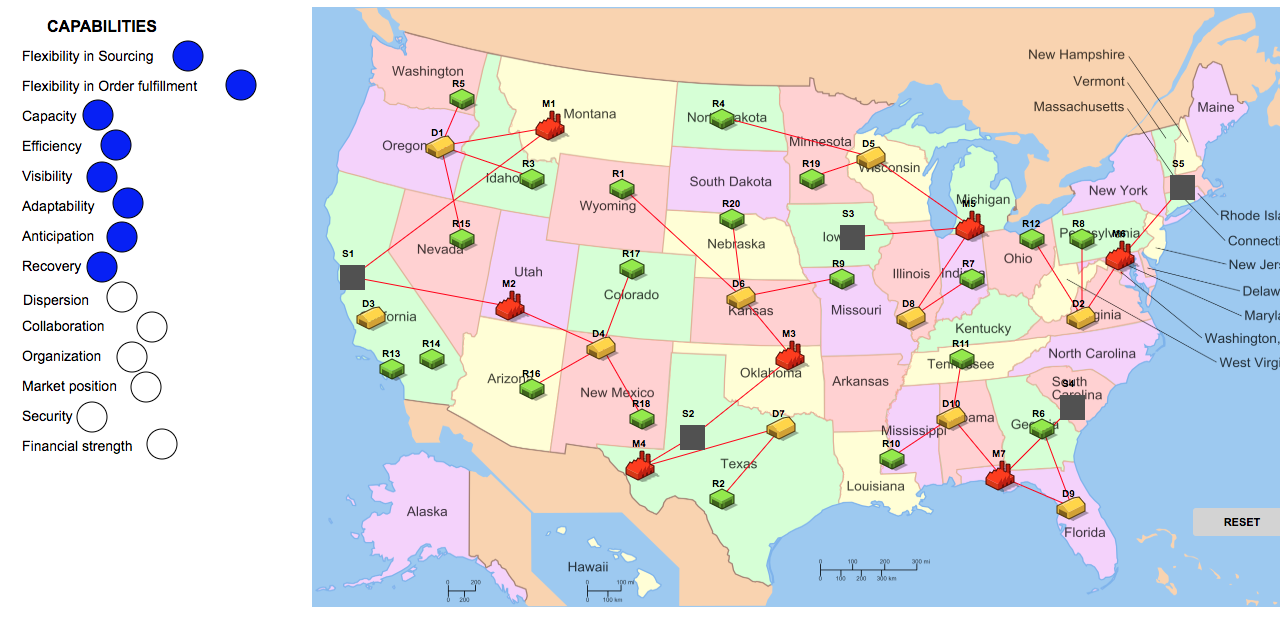
\includegraphics[width=6.5in]{figures/pdf/S3DLD.png}\\
  \caption{Scenario III (Distributor Level Disruption)}
  {The distributor D3 is getting disrupted due to which the retailers associated with it are left unsatisfied. The manufacturer facility M2 is holding the inventory required by the disrupted facility D3. The capabilities associated with this type of disruption are being identified.}
  \label{S3DL}
\end{figure}   

The Fig \ref{S3DL} exhibits the disruption occurring at the distributor facility D3. Due to this disruption, the retailers R13 and R14 along with the manufacturing facility M2 gets disconnected from D3. The retailers R13 and R14 have their demands unfulfilled due to this. There is a need for selecting an alternate source for distributor. This is made possible through the contingency planning component. The alternate distributor is selected in the similar manner as shown in \ref{ALTD}. The key indicator identification reduces the lost time ($T_{\text{L}}$) while the time for recovery ($T_{\text{R}}$) remains the same as that of equation \ref{3.8}. The resiliency of the system is improved by this reduction in time.

\begin{equation}
    Resiliency(R_S) = \frac{6}{18} = 33.33 \% \label{3.23}
\end{equation}

The resiliency and robustness considerations increase the resilience of the supply chain from 16.67 \% to 33.33 \% .

\begin{figure}[H]
  \centering
  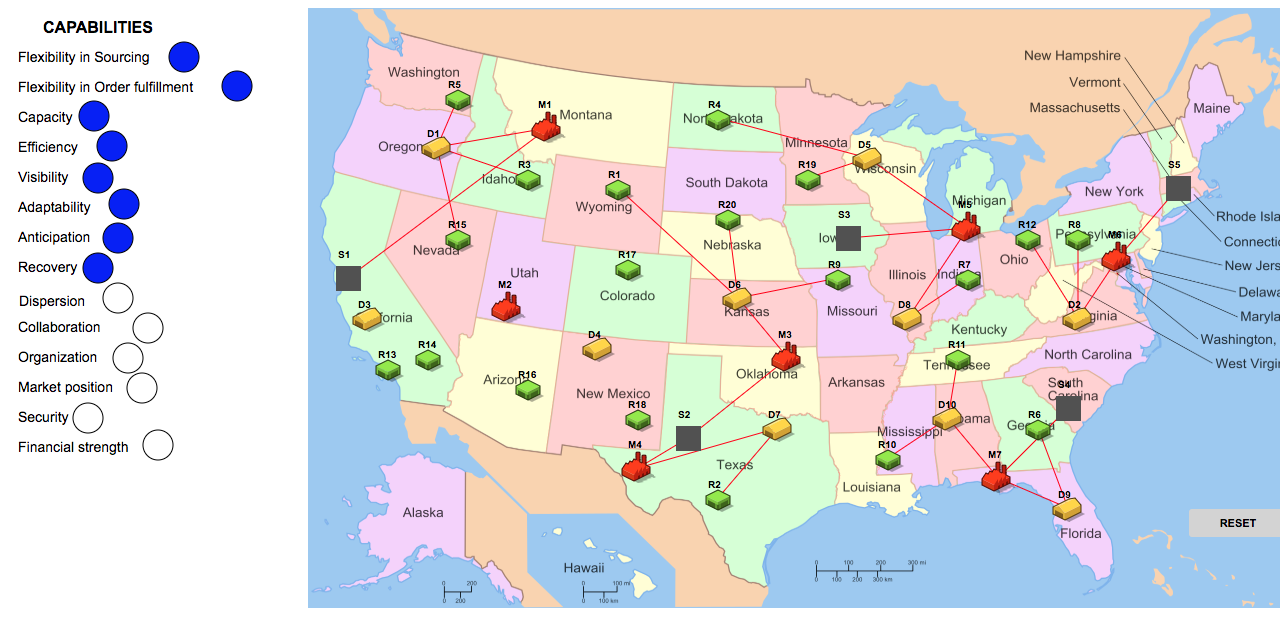
\includegraphics[width=6.5in]{figures/pdf/S3MLD.png}\\
  \caption{Scenario III (Manufacturer Level Disruption)}
  {The manufacturer M2 is getting disrupted due to which the  distributors and retailers associated with it are left unsatisfied. The supplier facility S1 is holding the inventory required by the disrupted facility M2. The capabilities associated with this type of disruption are being identified.}
  \label{S3ML}
\end{figure}   

In the Fig \ref{S3ML} the manufacturing facility M2 is disrupted thus causing the facilities linked with it to disconnect. The demands of the distributors and retailers linked with it are left dissatisfied. These distributors are relocated to a different manufacturer till the recovery of the M2 facility takes place. This relocation is done through the contingency planning component. The reduction in the lost time ($T_{\text{L}}$) through the identification component increases the resilience of the supply chain. The recovery time ($T_{\text{R}}$) is the same as equation \ref{3.9}. 

\begin{equation}
    Resiliency(R_S) = \frac{12}{54} = 22.23 \% \label{3.24}
\end{equation}

The resiliency and robustness considerations increase the resilience of the supply chain from 15.38 \% to 22.23 \% .

\begin{figure}[H]
  \centering
  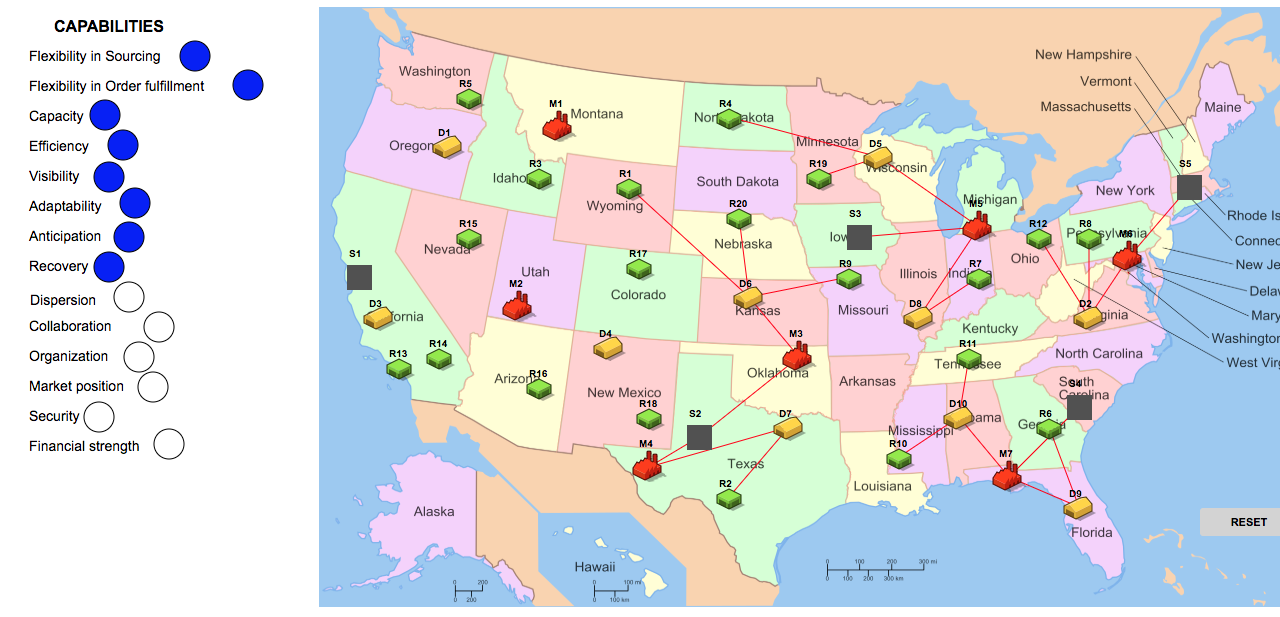
\includegraphics[width=6.5in]{figures/pdf/S3SLD.png}\\
  \caption{Scenario III (Supplier Level Disruption)}
   {The Supplier S1 is getting disrupted due to which the manufactures, distributors, and retailers are left unsatisfied. The entire supply chain is waiting for the facility S1 to be recovered for gaining back the functionality. The capabilities associated with this type of disruption are being identified.}
  \label{S3SL}
\end{figure}   

The Fig \ref{S3SL} depicts the disruption taking place at the supplier facility S1 in the supply chain. The whole supply chain has to wait on its recovery for receiving the materials as it is the sole supplier of the entire supply chain. The contingency planning component allots an alternate supplier facility to the manufacturers M1 and M2 associated with the supplier S1 and maintains a continuous flow of materials in the supply chain. The identification components brings down the lost time ($T_{\text{L}}$) while the recovery time ($T_{\text{R}}$) is the same as that of equation \ref{3.10}. There is an improvement observed in the resiliency of the supply chain because of this.

\begin{equation}
    Resiliency(R_S) = \frac{18}{96} = 18.75 \% \label{3.25}
\end{equation}

The resiliency and robustness considerations increase the resilience of the supply chain from 12.5 \% to 18.75 \%.

\subsubsection{SCENARIO IV: Disruptions due to Connectivity}

In this scenario, the supply chain face disruptions due to uncertainties in the connectivity. These arise from any complications in the scale of network, reliance upon information, and degree of outsourcing. The key indicators linked to this type of disruptions are the capabilities of visibility, adaptability, recovery, and security. The facilities at all the levels of disruption are kept the same. 

\subsubsection{Distributor Level disruption}

\begin{figure}[H]
  \centering
  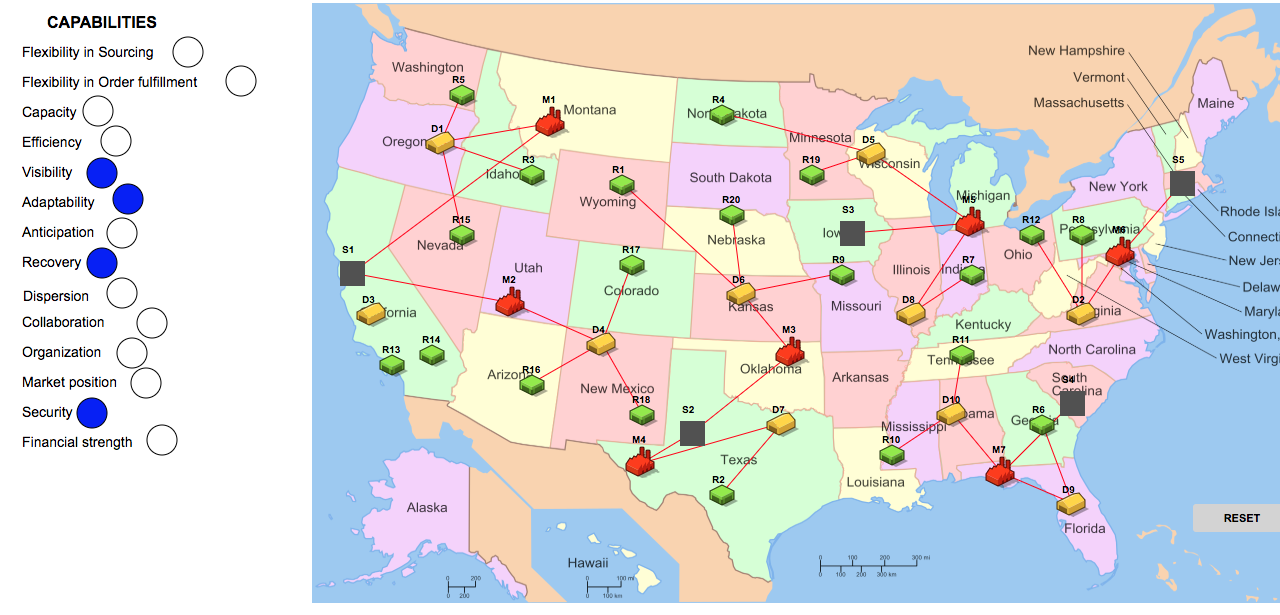
\includegraphics[width=6.5in]{figures/pdf/S4DLD.png}\\
  \caption{Scenario IV (Distributor Level Disruption)}
  {The distributor D3 is getting disrupted due to which the retailers associated with it are left unsatisfied. The manufacturer facility M2 is holding the inventory required by the disrupted facility D3. The capabilities associated with this type of disruption are being identified.}
  \label{S4DL}
\end{figure}   

The Fig \ref{S4DL} shows the distributed facility D3 and the effects it has on its linked facilities. The retailers R13 and R14 have to move to a different distributor for getting their demands satisfied. The contingency planning selects an alternate distributor facility for these retailers in the similar manner as shown in Fig \ref{ALTD}. The lost time ($T_{\text{L}}$) is reduced to 18 hours while the recovery time ($T_{\text{R}}$) remains the same as that of equation \ref{3.11}. The resiliency of the supply chain is then calculated as 

\begin{equation}
    Resiliency(R_S) = \frac{11}{18} = 61.11 \% \label{3.26}
\end{equation}

The resiliency and robustness considerations increase the resilience of the supply chain from 30.56 \% to 61.11 \%.

\begin{figure}[H]
  \centering
  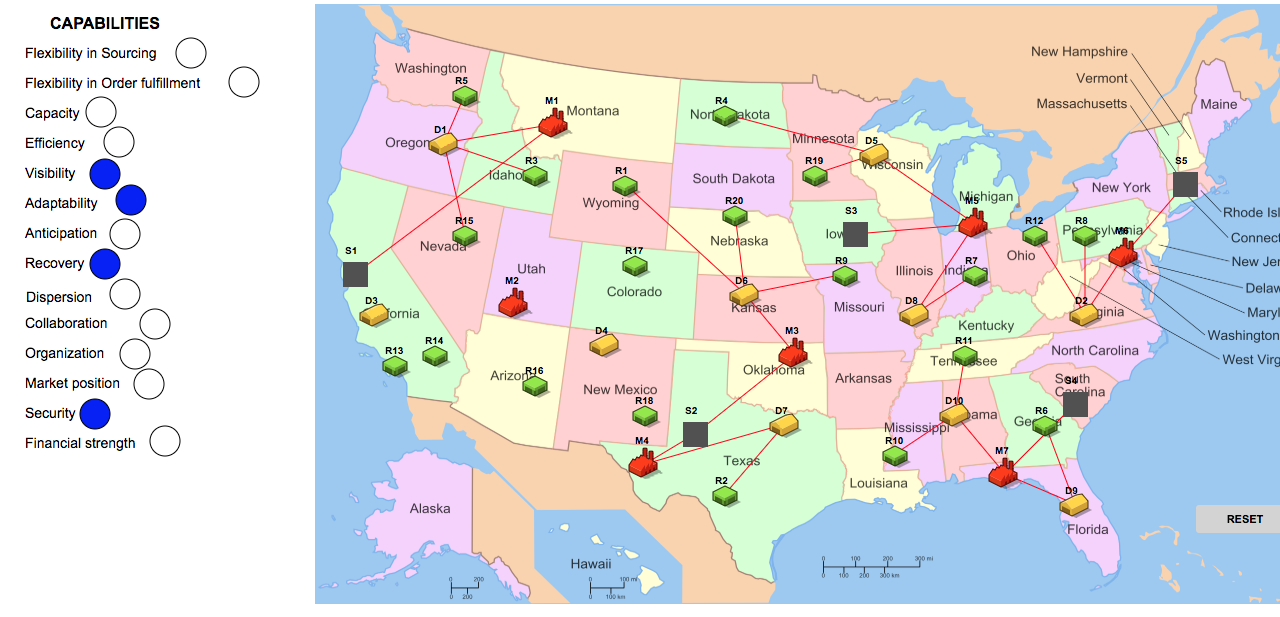
\includegraphics[width=6.5in]{figures/pdf/S4MLD.png}\\
  \caption{Scenario IV (Manufacturer Level Disruption)}
  {The manufacturer M2 is getting disrupted due to which the  distributors and retailers associated with it are left unsatisfied. The supplier facility S1 is holding the inventory required by the disrupted facility M2. The capabilities associated with this type of disruption are being identified.}
  \label{S4ML}
\end{figure}   

The disrupted manufacturer M2 is shown in Fig \ref{S4ML} along with the key indicators identification. This leads to the disconnection of D3 and D4 facilities to get disconnected from M2. Thus, the retailers associated with these distributors get affected. The alternate manufacturer is selected for these distributors with the help of contingency planning in the same way as shown in Fig \ref{ALTM} till the M2 facility recovers. The resiliency is increased by the incursion of key capabilities identification. The lost time ($T_{\text{L}}$) is reduced to 17 hours while the recovery time ($T_{\text{R}}$) remains the same as that of equation \ref{3.12}. 

\begin{equation}
    Resiliency(R_S) = \frac{17}{54} = 31.48 \% \label{3.27}
\end{equation}

The resiliency and robustness considerations increase the resilience of the supply chain from 21.79 \% to 31.48 \%.

\begin{figure}[H]
  \centering
  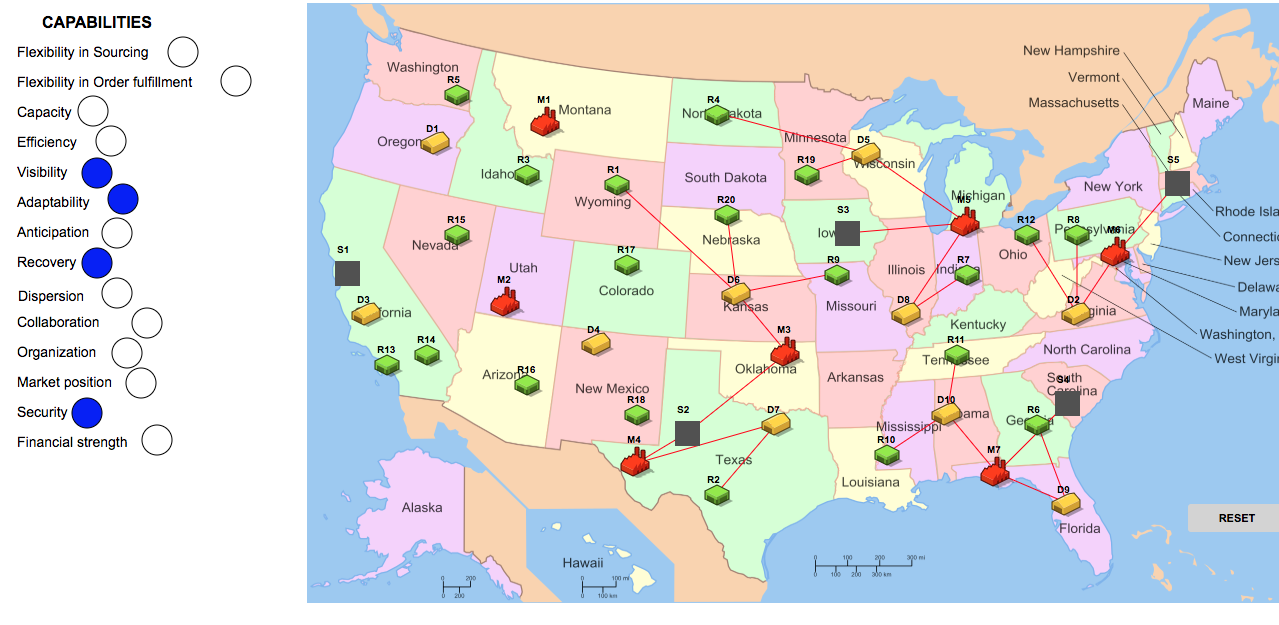
\includegraphics[width=6.5in]{figures/pdf/S4SLD.png}\\
  \caption{Scenario IV (Supplier Level Disruption)}
  {The Supplier S1 is getting disrupted due to which the manufactures, distributors, and retailers are left unsatisfied. The entire supply chain is waiting for the facility S1 to be recovered for gaining back the functionality. The capabilities associated with this type of disruption are being identified.}
  \label{S4SL}
\end{figure}  

The Fig \ref{S4SL} shows the supplier S1 being disrupted and the key indicators being identified. The contingency planning allocates a new supplier for the manufacturing facilities M1 and M2 which are completely reliant on the S1 facility. The new supplier is selected for M1 and M2 in the same way as shown in Fig \ref{ALTS}. The lost time ($T_{\text{L}}$) is reduced to 23 hours due to the identification component while the recovery time ($T_{\text{R}}$) remains the same as that of equation \ref{3.13}.

\begin{equation}
    Resiliency(R_S) = \frac{23}{96} = 23.95 \% \label{3.28}
\end{equation}

The resiliency and robustness considerations increase the resilience of the supply chain from 15.79 \% to 23.95 \%.

\subsubsection{SCENARIO V: Disruptions due to Deliberate Threats}

In this scenario, the disruption in the supply chain is caused due to the deliberate threats. These disruptions occur mainly due to labor disputes, theft, and terrorism/sabotage. The key capabilities associated with this type of disruption are identified as security, anticipation, and collaboration. The facilities which get affected are the same at all levels of disruptions in the supply chain.

\subsubsection{Distributor Level Disruption}

\begin{figure}[H]
  \centering
  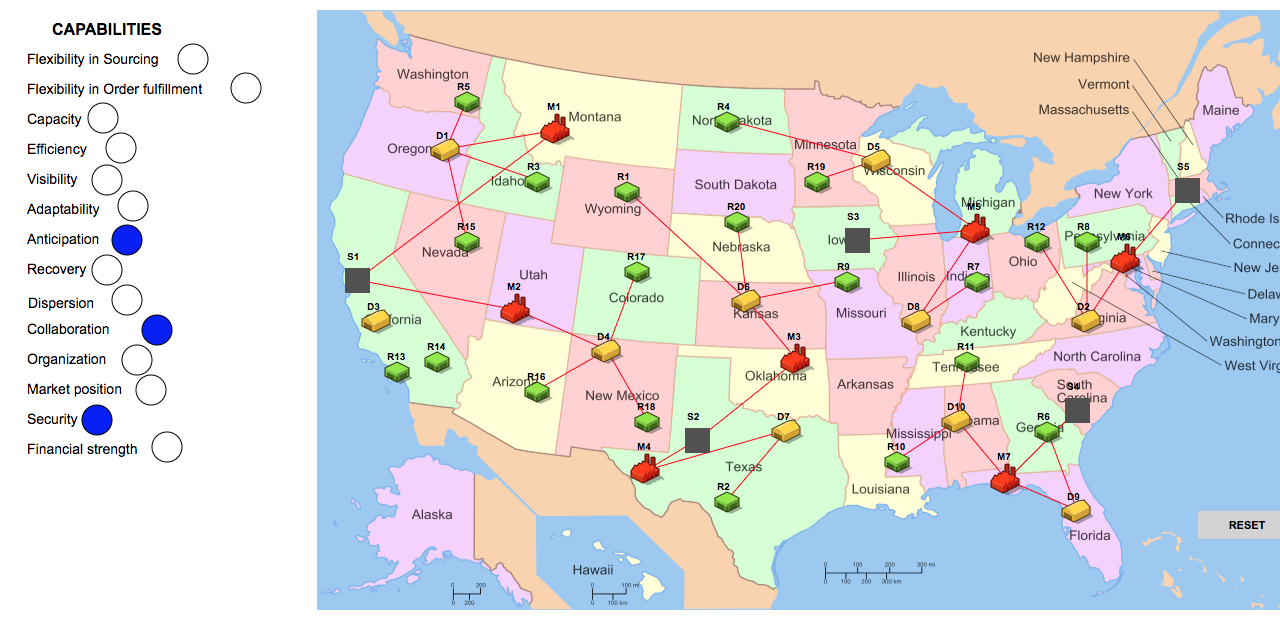
\includegraphics[width=6.5in]{figures/pdf/S5DLD.png}\\
  \caption{Scenario V (Distributor Level Disruption)}
  {The distributor D3 is getting disrupted due to which the retailers associated with it are left unsatisfied. The manufacturer facility M2 is holding the inventory required by the disrupted facility D3. The capabilities associated with this type of disruption are being identified.}
  \label{S5DL}
\end{figure}   
 
The Fig \ref{S5DL} displays the distributor facility D3 being disrupted and the key indicators being identified. The retailers R13 and R14 along with the manufacturer M2 get disconnected from the D3 facility. The contingency planning component allocates a different distributor facility in the same way as shown in Fig \ref{ALTD} while the disrupted D3 facility is recovered. The lost time ($T_{\text{L}}$) is reduced to 18 hours while the recovery time ($T_{\text{R}}$) is the same as that of equation \ref{3.14}. The resiliency of the supply chain is thus found out as

\begin{equation}
    Resiliency(R_S) = \frac{10}{18} = 55.55 \% \label{3.29}
\end{equation}

The resiliency and robustness considerations increase the resilience of the supply chain from 27.78 \% to 55.55 \%.

\begin{figure}[H]
  \centering
  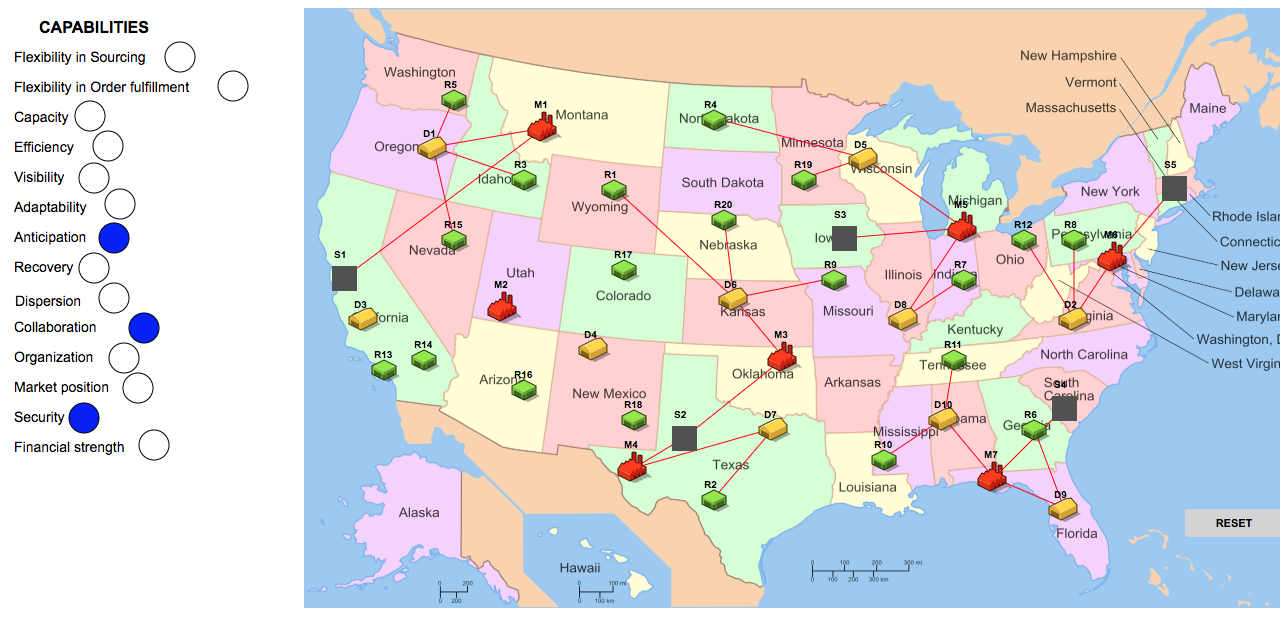
\includegraphics[width=6.5in]{figures/pdf/S5MLD.png}\\
  \caption{Scenario V (Manufacturer Level Disruption)}
  {The manufacturer M2 is getting disrupted due to which the  distributors and retailers associated with it are left unsatisfied. The supplier facility S1 is holding the inventory required by the disrupted facility M2. The capabilities associated with this type of disruption are being identified.}
  \label{S5ML}
\end{figure}   

The manufacturing facility M2 is disrupted and the key capabilities are indicated as shown in the Fig \ref{S5ML}. The contingency planning selects an alternate manufacturing facility for the distributors D3 and D4 which are associated with the disrupted facility M2. This is selection is done similar to that as shown in the Fig \ref{ALTM} while the disrupted facility recovers. The identification element decreases the lost time ($T_{\text{L}}$) to 16 hours while the recovery time ($T_{\text{R}}$) remains the same as that of equation \ref{3.15}. The resiliency value of the supply chain is calculated as

\begin{equation}
    Resiliency(R_S) = \frac{16}{54} = 29.62 \% \label{3.30}
\end{equation}

The resiliency and robustness considerations increase the resilience of the supply chain from 20.54 \% to 29.62 \%.

\begin{figure}[H]
  \centering
  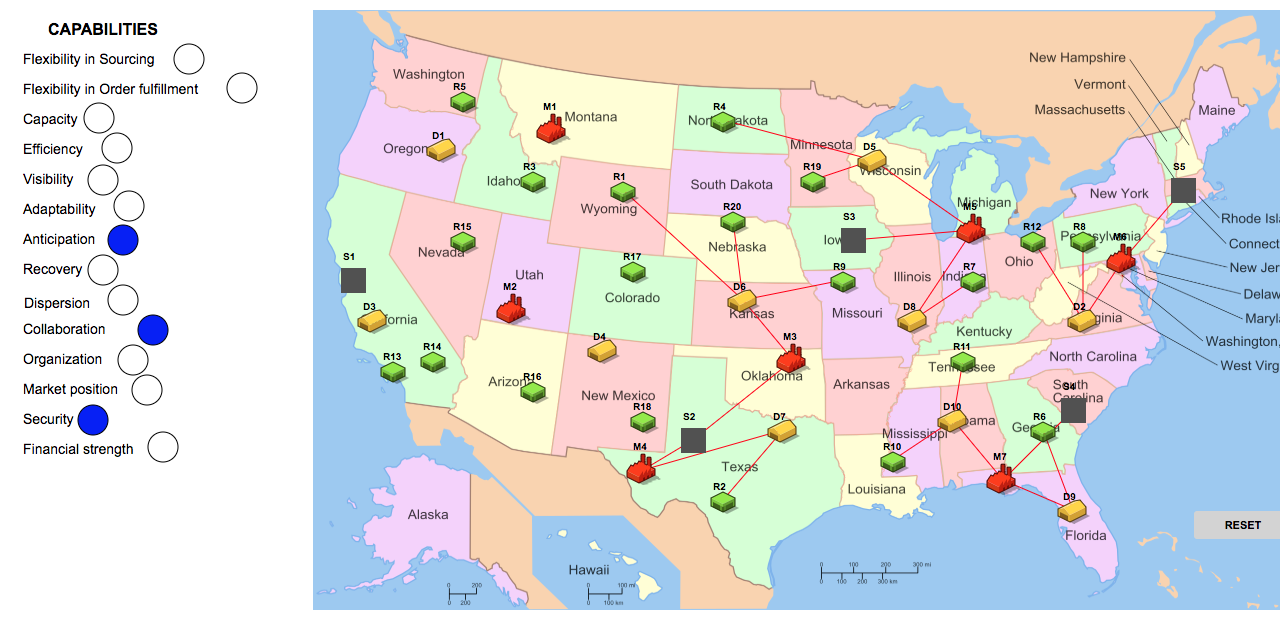
\includegraphics[width=6.5in]{figures/pdf/S5SLD.png}\\
  \caption{Scenario V (Supplier Level Disruption)}.
  {The Supplier S1 is getting disrupted due to which the manufactures, distributors, and retailers are left unsatisfied. The entire supply chain is waiting for the facility S1 to be recovered for gaining back the functionality. The capabilities associated with this type of disruption are being identified.}\label{S5SL}
\end{figure}  

In the Fig \ref{S5SL} the disrupted supplier facility S1 is displayed along with the key indicators being identified at the time of the disruption. Alternate supplier facility for the manufacturers M1 and M2 is done through contingency planning so that the continuous supply chain is achieved. This supplier is selected the same way as shown in the Fig \ref{ALTS}. The resiliency is improved by the application of the identification element in the supply chain. The lost time ($T_{\text{L}}$) is lowered to 22 hours while the recovery time ($T_{\text{R}}$) remains the same as that of equation \ref{3.16}. The supply chain resiliency is then given as

\begin{equation}
    Resiliency(R_S) = \frac{22}{96} = 22.91 \% \label{3.31}
\end{equation}

The resiliency and robustness considerations increase the resilience of the supply chain from 15.27 \% to 22.91 \%.

The resiliency values for all the scenarios at all the levels right from the equation \ref{3.2} to equation \ref{3.31} are accrued together and are put in a tabular form and are shown in the Fig \ref{RESV} for observing the improvements in the supply chain resiliency before and after the consideration of resiliency and robustness

\begin{figure}[H]
  \centering
  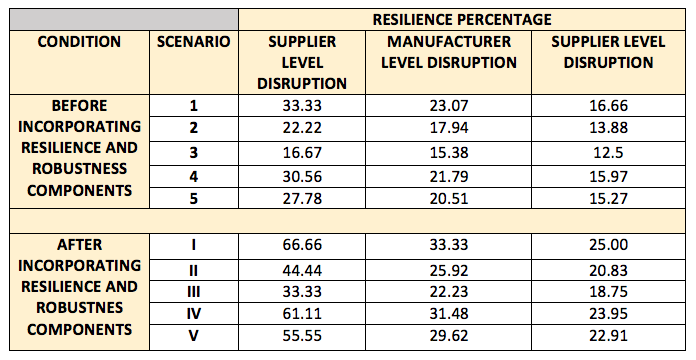
\includegraphics[width=6.5in]{figures/pdf/ResilienceValues.png}\\
  \caption{All the Resilience values}\label{RESV}
\end{figure}  



\begin{figure}[H]
  \centering
  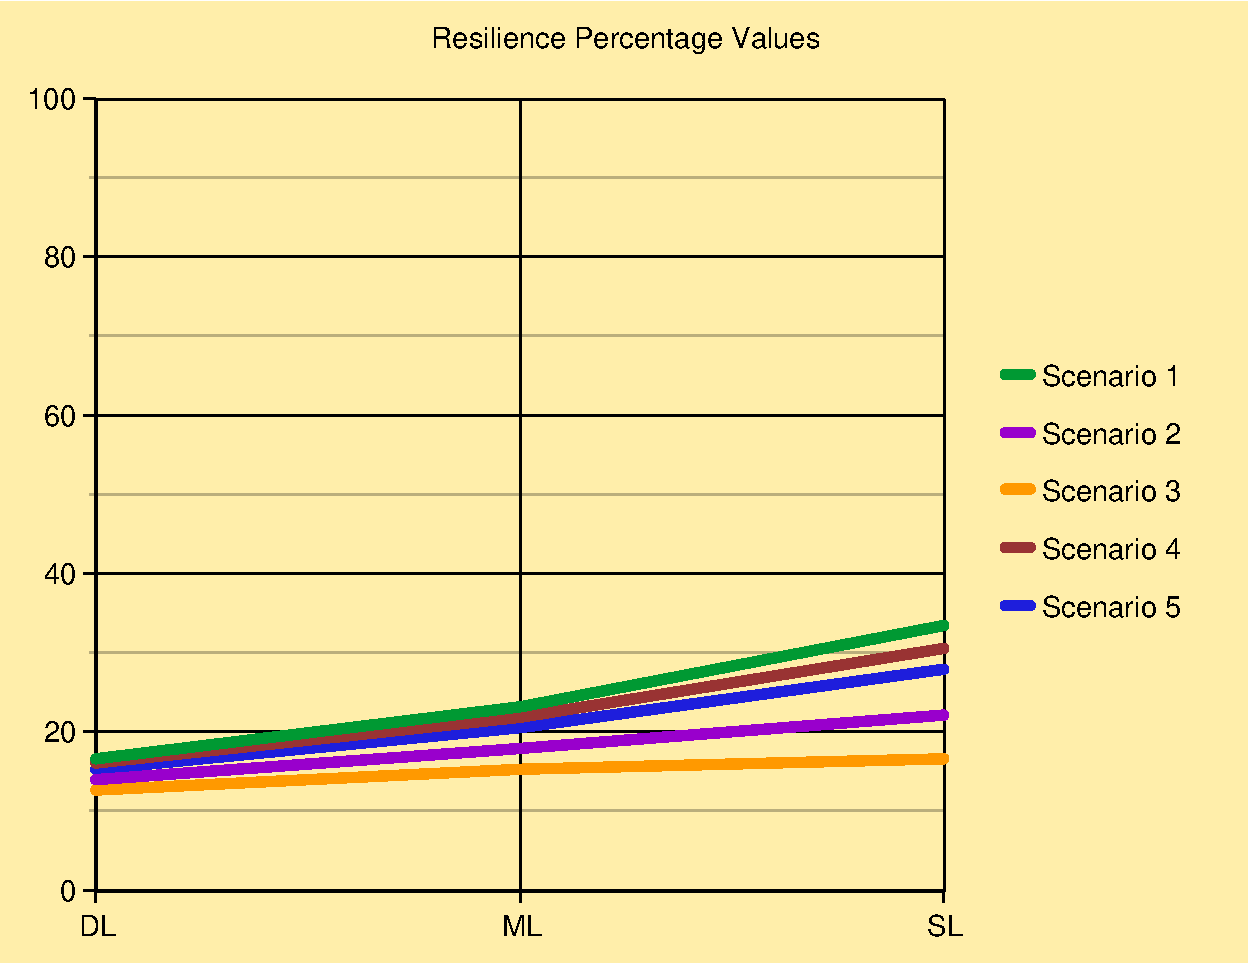
\includegraphics[width=5.5in]{figures/pdf/Before(Graph).pdf}\\
  \caption{Graph for the Resiliency values for the Supply Chain before incorporating Resilience and Robustness Components}\label{G1}
\end{figure}  

It is clearly evident that there is an improvement in all the scenarios after the inclusion on resilience and robustness components in the design of the supply chain. These values when plotted on a graph describe the difference between the two strategies very efficiently. The Fig \ref{G1}shows the graph of the values of all the values of the resiliency obtained before including the resiliency and robustness components. After these components are included in the supply chain, the resilience percentage values increase for the disruptions occurring at all the levels. This can be seen from the graph in Fig \ref{G2}.

\begin{figure}[H]
  \centering
  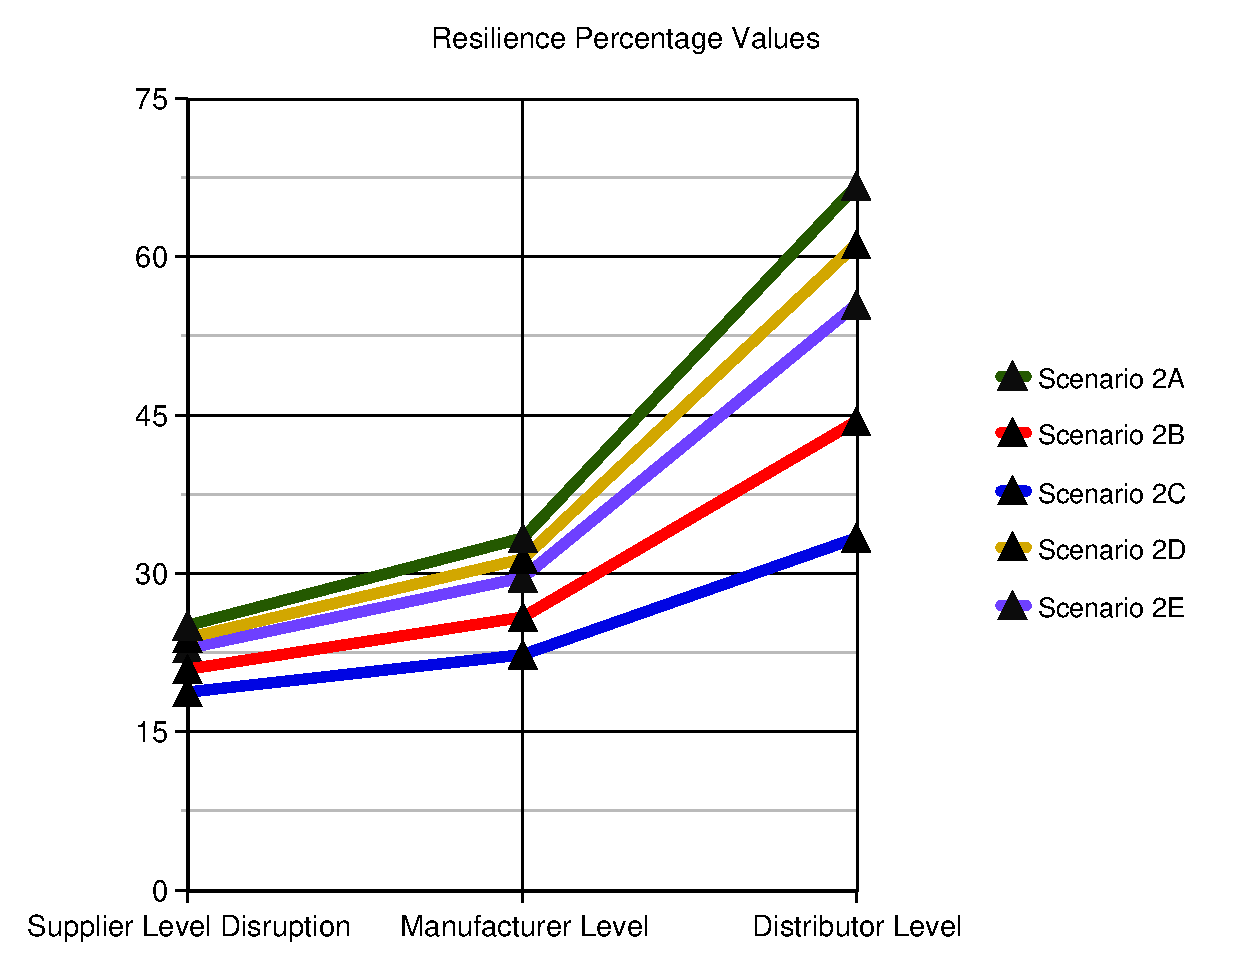
\includegraphics[width=5.5in]{figures/pdf/After(Graph).pdf}\\
  \caption{Graph for the Resiliency values for the Supply Chain after incorporating Resilience and Robustness Components}\label{G2}
\end{figure}  